\documentclass[11pt,a4paper,openany]{report}
\usepackage[T1]{fontenc}
\usepackage[utf8]{inputenc}
\usepackage{lmodern}
\usepackage{microtype}
\usepackage{amsmath,amssymb,amsthm,mathtools,bm}
\usepackage{booktabs,array,longtable,tabularx}
\usepackage{xcolor}
\usepackage[margin=24mm,headheight=23pt]{geometry}
\usepackage{enumitem}
\usepackage{fancyhdr}
\usepackage{fancyvrb}
\usepackage{graphicx}
\usepackage{url}
\usepackage{xurl}
\usepackage{hyperref}

\definecolor{finblue}{HTML}{1F5A99}
\definecolor{fingreen}{HTML}{19733A}
\definecolor{finorange}{HTML}{D55E00}
\definecolor{finred}{HTML}{A61B1B}
\definecolor{finviolet}{HTML}{6A3D9A}

\hypersetup{
  unicode=true,
  colorlinks=true,
  linkcolor=finblue,
  citecolor=fingreen,
  urlcolor=finblue,
  pdftitle={FIN Programs 217--229: Operational Sections, Reference Costs, and Heat-Kernel Spectral Tomography},
  pdfauthor={Krzysztof Żuchowski},
  pdfsubject={Operational central states, exponent no-go, symmetry-reference costs, moment bounds, formal cores, and heat-kernel spectral tomography},
  pdfkeywords={FIN, spectral theory, operational tomography, heat kernel, bistochastic state, asymmetry resource, fidelity, e-process, trigonometric moment problem}
}

\pagestyle{fancy}
\fancyhf{}
\fancyhead[L]{\small FIN Programs 217--229}
\fancyhead[R]{\small Release 10.20}
\fancyfoot[C]{\thepage}
\setlength{\parindent}{0pt}
\setlength{\parskip}{0.55em}
\setlist{nosep,leftmargin=2em}
\setcounter{tocdepth}{2}
\setcounter{secnumdepth}{3}
\emergencystretch=3em

\newcommand{\one}{\bm 1}
\newcommand{\C}{\mathbb C}
\newcommand{\R}{\mathbb R}
\newcommand{\Z}{\mathbb Z}

\begin{document}
\hypersetup{pageanchor=false}
\begin{titlepage}
\centering
\vspace*{8mm}
{\Large\bfseries FIN Research Monograph --- Release 10.20\par}
\vspace{10mm}
{\Huge\bfseries FIN Programs 217--229\par}
\vspace{6mm}
{\Large Operational Sections, Reference Costs,\\
and Heat-Kernel Spectral Tomography\par}
\vspace{16mm}
{\Large Krzysztof \.Zuchowski\par}
\vspace{2mm}
{\normalsize Independent Researcher --- Fractal Information Theory Project\par}
\vspace{2mm}
{\normalsize ORCID: \href{https://orcid.org/0009-0002-0909-3613}{0009-0002-0909-3613}\par}
\vspace{10mm}
{\large 27 July 2026\par}
{\normalsize Publication --- Preprint; record version 1.0.0\par}
\vfill
\begin{minipage}{0.88\textwidth}
\small
\textbf{Scope.} Thirteen executed studies of operational central states,
natural exponent flows, formal certification, finite symmetry-reference
costs, dependence-aware inference, process tomography, environmental moments,
phase formalization, heat-kernel spectral reconstruction, independent
custody, and external prediction gating.

\medskip
\textbf{Central result.} Exact heat transition data identify the finite
generator by \(A=-\tau^{-1}\log P_\tau\), while projective eigenvalue ratios
remain identifiable without an absolute clock unit. Imperfect symmetry
references cannot be returned in uncorrelated product form after broadcasting
nonzero asymmetry.

\medskip
\textbf{Guardrail.} No QW-2191 discharge, strict selector, canonical physical
unit, target-independent strict exponent source, completed legacy--strict
bridge, role transfer, \(L_{\rm total}\), external physical validation, or
Theory-of-Everything closure is claimed.

\medskip
\textbf{License.} Creative Commons Attribution 4.0 International (CC BY 4.0).
\end{minipage}
\vfill
\end{titlepage}
\hypersetup{pageanchor=true}

\pagenumbering{roman}
\chapter*{Publication statement}
\addcontentsline{toc}{chapter}{Publication statement}
This release reports Programs 217--229 and recommends Programs 230--242.
Analytic proofs, exact arithmetic, machine-checked finite fragments,
simulation evidence, conditional instruments, unavailable infrastructure,
and failed external-data gates remain separate.

\tableofcontents
\clearpage
\pagenumbering{arabic}

\section{Confidence convention}

The report distinguishes analytic proof, exact arithmetic, machine-checked finite fragments, simulation evidence, conditional operational construction, and open infrastructure or data gates. No finite example or unavailable external test is promoted.

\chapter{Abstract}

This monograph reports thirteen executed research programs, numbered 217 through 229. They continue the axiomatic and operational analysis of the dimensionless FIN spectral framework after Programs 204--216 established that a self-adjoint generator does not by itself select a central state, an orientation reference, a dimensional clock, or an independent experimental record.

Program 217 identifies the exact morphism boundary of the proposed central state. The uniform probability vector is fixed by every bistochastic sector channel, and invariance under the permutation subcategory makes it unique. For sector dimensions \((1,2,2,2,2)\) the corresponding expectation is \(9/5\). In contrast, a nonuniform preparation law is selected operationally by observed frequencies. A simultaneous Hoeffding theorem quantifies this frequency section without turning it into a strict source.

Program 218 proves an affine-naturality obstruction for the strict damping exponent. In the coordinate \(x=\eta-1\), every continuous vector field satisfying

\[
F(ax)=aF(x),
\qquad a>0,
\]

and reflection oddness has the form \(F(x)=\kappa x\). If \(\kappa\ne0\), its only fixed point is zero; if \(\kappa=0\), every point is fixed. Therefore the nonzero strict increment \(x=4/5\) cannot be uniquely selected by such a flow. An exact polynomial audit through degree eight has rank eight, nullity one, and leaves only the linear monomial.

Program 221 develops a quantitative resource theorem for the missing orientation. When no second asymmetric source is consumed, an imperfect reference

\[
\kappa_r=\frac{I+r\sigma_x}{2},
\qquad 0\le r<1,
\]

cannot produce a nonzero asymmetric target and be returned exactly, uncorrelated with that target. The reflected pair has squared fidelity \(1-r^2\), whereas the ideal product output has fidelity \((1-r^2)(1-t^2)\). Monotonicity of fidelity under channels gives an exact no-broadcast theorem. If product return is relaxed to marginal return, an explicit covariant measure-and-prepare channel succeeds by storing correlations. For \(r=0.8\) and target asymmetry \(t=0.6\), the required mutual information is \(0.178364\) bits. The construction quantifies a supplied selector resource; it does not source its sign or discharge QW-2191.

Programs 222--224 improve the statistical layer. A robust integer optimization of thinning lag and failure-budget allocation reduces the valid hidden-mixing DKW radius from \(0.203960\) to \(0.199102\) while including uncertainty in a separately calibrated refresh rate. Sequential insertion ranks yield an exact reusable-calibration e-process in the filtration generated by those ranks. A likelihood-quadratic process region reduces tomography widths by approximately one half and attains empirical coverage \(0.956667\), but it is explicitly retained as an asymptotic method rather than an exact finite-sample confidence theorem.

Program 225 solves the next trigonometric moment problem exactly. Given

\[
c_1=\frac45,
\qquad
c_2=\frac12,
\]

positive semidefiniteness of the order-three Toeplitz matrix is equivalent to

\[
-\frac{11}{180}\le c_3\le\frac{11}{20}.
\]

Both endpoints are attained by explicit symmetric atomic phase measures. This bounds one more operational environmental observable without choosing a unique microscopic environment.

Programs 220 and 226 advance formal verification in a deliberately scoped way. Two dependency-free Lean 4 sources compile locally. One verifies constant null modes, two independent four-cycle energy formulas, the exact archived energy \(30\), and its nonnegativity. The other verifies the complete order-eight residue orbit and \(\gcd(743,4000)=1\). The general Mathlib-dependent graph library and the analytic automatic-continuity and transcendence arguments remain uncompiled. Arb/\allowbreak{}python-flint also remains unavailable; no fractional certificate is promoted.

The principal physics-bridge result is Program 227. It constructs an explicit heat-kernel tomography instrument: prepare every vertex basis state, evolve for one positive duration \(\tau\), and measure the vertex POVM. Exact transition probabilities determine

\[
P_\tau=e^{-\tau A},
\qquad
A=-\frac1\tau\log P_\tau.
\]

Even before a dimensional clock is supplied, the projective eigenvalue ratios of \(A\) are identifiable from the logarithms of the eigenvalues of \(P_\tau\). In finite-shot simulations, the frozen strict spectral fingerprint passes in \(3.75\%\), \(72.9\%\), and \(100\%\) of trials at respectively 2,000, 10,000, and 50,000 shots per preparation.

No independent eleven-field process or double-slit event bundle is present. The external semigroup prediction

\[
P_{2\tau}^{\rm predicted}=P_\tau^2
\]

is preregistered but correctly not executed. No strict central state, target-independent \(\eta\) source, formal Arb closure, complete Mathlib library, non-premise selector, canonical physical unit, legacy-to-strict bridge, role transfer, \(L_{\rm total}\), external validation, or Theory-of-Everything closure is claimed.

\par\medskip\hrule\medskip

\chapter{Executive summary}

\section{Outcome table}

\begin{center}
\begingroup\small
\setlength{\tabcolsep}{3.5pt}
\renewcommand{\arraystretch}{1.16}
\begin{longtable}{@{}p{0.067\textwidth}p{0.409\textwidth}p{0.244\textwidth}p{0.140\textwidth}@{}}
\toprule
\textbf{Program} & \textbf{Constructed object} & \textbf{Result} & \textbf{Confidence} \\
\midrule
\endhead
217 & BistochasticCentralStateAndFrequencySection & uniform categorical state separated from empirical preparation state & Proven \\
218 & AffineNaturalEtaVectorFieldNoGo & affine-natural flows cannot select \(4/5\) & Proven \\
219 & ArbExecutionAttestation & formal engine remains unavailable & Proven environment audit \\
220 & ScopedLeanDirichletBuild & exact C4 core compiles; general Mathlib theorem remains open & Machine checked in scope \\
221 & CorrelatedReferenceLedger & imperfect exact product catalysis is impossible; marginal return requires correlations & Proven \\
222 & RobustMixingDesignOptimizer & calibrated robust DKW design improved & Proven bound; finite optimization \\
223 & SequentialInsertionRankEProcess & calibration-reusing rank e-process constructed & Proven in rank filtration \\
224 & LikelihoodQuadraticProcessRegion & narrower tomography region with model control & Strong evidence; asymptotic \\
225 & ThirdMomentToeplitzInterval & sharp \(c_3\) interval with endpoint measures & Proven \\
226 & ScopedPhaseFormalizationRecord & finite torsion core compiles; analytic hierarchy remains & Machine checked in scope \\
227 & HeatKernelTomographyInstrument & exact instrument-to-spectrum identifiability & Proven; finite-shot evidence \\
228 & IndependentCustodyBundleV2 & acquisition schema strengthened; no bundle admitted & Proven local audit \\
229 & SemigroupHoldoutPredictionLock & external prediction frozen and locked & Proven gate status \\
\bottomrule
\end{longtable}
\endgroup
\end{center}

\section{Central advance}

The most important advance is not another internal kernel identity. It is the construction of a complete conditional observation map

\[
\text{preparations}
\longrightarrow
P_\tau
\longrightarrow
\operatorname{spec}(A)/\mathbb R_+
\longrightarrow
\text{frozen spectral fingerprint}.
\]

Programs 189, 201, and 214 established that projective spectral information survives the absence of an absolute unit. Program 227 now proves how a declared instrument can reconstruct that information. The remaining bridge to physics is no longer the vague instruction "measure the operator." It is the concrete obligation to supply:

\begin{enumerate}
\item 
vertex-basis or informationally complete preparations;

\item 
a calibrated evolution duration;

\item 
a vertex-resolving measurement;

\item 
finite-shot transition counts;

\item 
an independent custody and holdout protocol.

\end{enumerate}

The first four form a mathematical instrument model. The fifth is still absent as an empirical object.

\section{Exact new theorems}

Four theorem-level results deserve emphasis.

\subsection{Theorem A --- operational central-state dichotomy}

The only probability vector fixed by every permutation of \(m\) sectors is \(u=(1/m,\ldots,1/m)\). Since permutation matrices are bistochastic, a state fixed by all bistochastic endomorphisms is uniquely uniform. A nonuniform central state can nevertheless be selected by an explicit preparation distribution and estimated with a distribution-free frequency band.

\subsection{Theorem B --- affine-natural exponent no-go}

Every continuous, positively one-homogeneous, odd vector field on a one-dimensional real representation is linear. It has no unique nonzero fixed point. Thus the exponent increment \(4/5\) requires a new non-affine or scale-bearing datum.

\subsection{Theorem C --- imperfect-reference no-broadcast}

An imperfect finite \(\mathbb Z_2\) reference cannot be returned exactly in product form after generating any nonzero asymmetry, unless another asymmetric input is consumed. Correlated marginal return remains possible.

\subsection{Theorem D --- heat-instrument spectral reconstruction}

For symmetric positive semidefinite \(A\) and known \(\tau>0\), \(P_\tau=e^{-\tau A}\) is symmetric positive definite and has a unique real principal logarithm. Therefore \(A=-\tau^{-1}\log P_\tau\). If \(\tau\) is not dimensionally calibrated, the ratios \(\lambda_k/\lambda_{\max}\) are still determined.

\section{Honest failures}

\begin{itemize}
\item 
The uniform categorical state still depends on the bistochastic morphism premise.

\item 
No target-independent exponent law selects \(9/5\).

\item 
Arb and python-flint remain unavailable.

\item 
The general graph theorem still lacks Mathlib compilation.

\item 
The reference-resource theorem does not source the first orientation sign.

\item 
The improved tomography ellipsoid is not exact finite-sample inference.

\item 
The analytic phase theorem is not fully machine formalized.

\item 
No independent process or double-slit record exists locally.

\item 
The external prediction remains unexecuted.

\end{itemize}

These are retained as scientific outcomes rather than concealed by a new interpretation.

\par\medskip\hrule\medskip

\chapter{Scope and guardrails}

\section{Kernel separation}

The legacy intermediate kernel remains

\[
K_{\rm legacy}(d)=
\alpha_{\rm geo}
\frac{\cos(\omega_\ell d+\phi_\ell)}
{1+\beta_{\rm tors}d},
\]

with

\[
\alpha_{\rm geo}=4\ln2,
\qquad
\omega_\ell=\frac\pi4,
\qquad
\phi_\ell=\frac\pi6,
\qquad
\beta_{\rm tors}=0.01,
\]

whereas the later strict working kernel is

\[
K_{\rm strict}(d)=
\frac{\cos(\omega_s d+\phi_s)}
{1+\beta_s d^{\eta_s}},
\]

with

\[
\omega_s=0.18575,
\qquad
\phi_s=0.16250,
\qquad
\beta_s=1,
\qquad
\eta_s=\frac95.
\]

The studies do not identify these two kernels. Program 218 attacks only the possibility that a natural exponent flow selects the strict exponent. Program 227 uses only the frozen strict finite operator as the target of an operational fingerprint. Neither action starts legacy role transfer.

\section{Spectral core}

For a symmetric nonnegative weight matrix \(W\) with constant row sum \(s\),

\[
A=sI-W
\]

satisfies

\[
\langle f,Af\rangle
=
\frac12\sum_{x,y}W_{xy}|f_x-f_y|^2\ge0.
\]

The same generator gives

\[
U_t=e^{-itA},
\qquad
P_t=e^{-tA},
\qquad
G_z=(A+zI)^{-1}.
\]

These wave, diffusion, and Green representations remain mathematically unified. The present round studies which additional objects are needed to observe them.

\section{Claim levels}

\begin{itemize}
\item 
\textbf{Proven:} analytic proof or exact arithmetic.

\item 
\textbf{Machine checked in scope:} a named finite proposition compiled by Lean.

\item 
\textbf{Strong evidence:} reproducible finite simulation or numerical audit.

\item 
\textbf{Conditional:} the result requires an explicit preparation, calibration, apparatus, environment, or external record.

\item 
\textbf{Open:} a required toolchain, source theorem, or dataset is absent.

\end{itemize}

No simulation is promoted to a theorem. No compiled example is promoted to a general formal library. No data schema is promoted to an experiment.

\par\medskip\hrule\medskip

\chapter{Program 217 --- Central states as operational sections}

\section{Bistochastic category}

Let the central state space be the simplex

\[
\Delta_{m-1}
=
\left\{p\in\mathbb R^m:
p_i\ge0,\ \sum_i p_i=1
\right\}.
\]

A bistochastic sector channel is a matrix \(T\) satisfying

\[
T_{ij}\ge0,
\qquad
T\mathbf1=\mathbf1,
\qquad
\mathbf1^\mathsf TT=\mathbf1^\mathsf T.
\]

The uniform state \(u=\mathbf1/m\) obeys \(Tu=u\).

Conversely, suppose \(p\) is fixed by every permutation matrix. Transpositions give \(p_i=p_j\) for every pair, hence \(p=u\). Thus uniformity is already unique under the permutation subcategory and remains unique under the larger bistochastic category.

Four hundred random convex combinations of permutation matrices give a maximum invariance residual

\[
8.33\times10^{-17}.
\]

For \((d_i)=(1,2,2,2,2)\),

\[
\sum_i u_i d_i=\frac95.
\]

\section{Preparation-frequency section}

An apparatus may prepare central sectors according to a nonuniform law. The challenge distribution was

\[
p=(0.10,0.15,0.20,0.25,0.30),
\]

whose dimension expectation is \(1.9\), not \(1.8\).

For \(n\) independent preparation labels with empirical frequencies \(\widehat p\), the union bound and Hoeffding inequality give

\[
\Pr\left(
\|\widehat p-p\|_\infty>\varepsilon
\right)
\le
2m e^{-2n\varepsilon^2}.
\]

At \(m=5\), \(n=5000\), and \(\delta=0.05\), the simultaneous radius is

\[
\varepsilon=
\sqrt{\frac{\log(2m/\delta)}{2n}}
=
0.0230181.
\]

All 600 declared simulations cover.

\section{Interpretation}

The categorical theorem answers "which state is invariant?" The frequency theorem answers "which state was prepared?" These are different questions. The second can be measured without being forced by the first.

\textbf{Verdict --- Proven.} The morphism class fixes uniformity conditionally; preparation data supply nonuniform weights operationally. No strict state source is exported.

\begin{figure}[htbp]
\centering
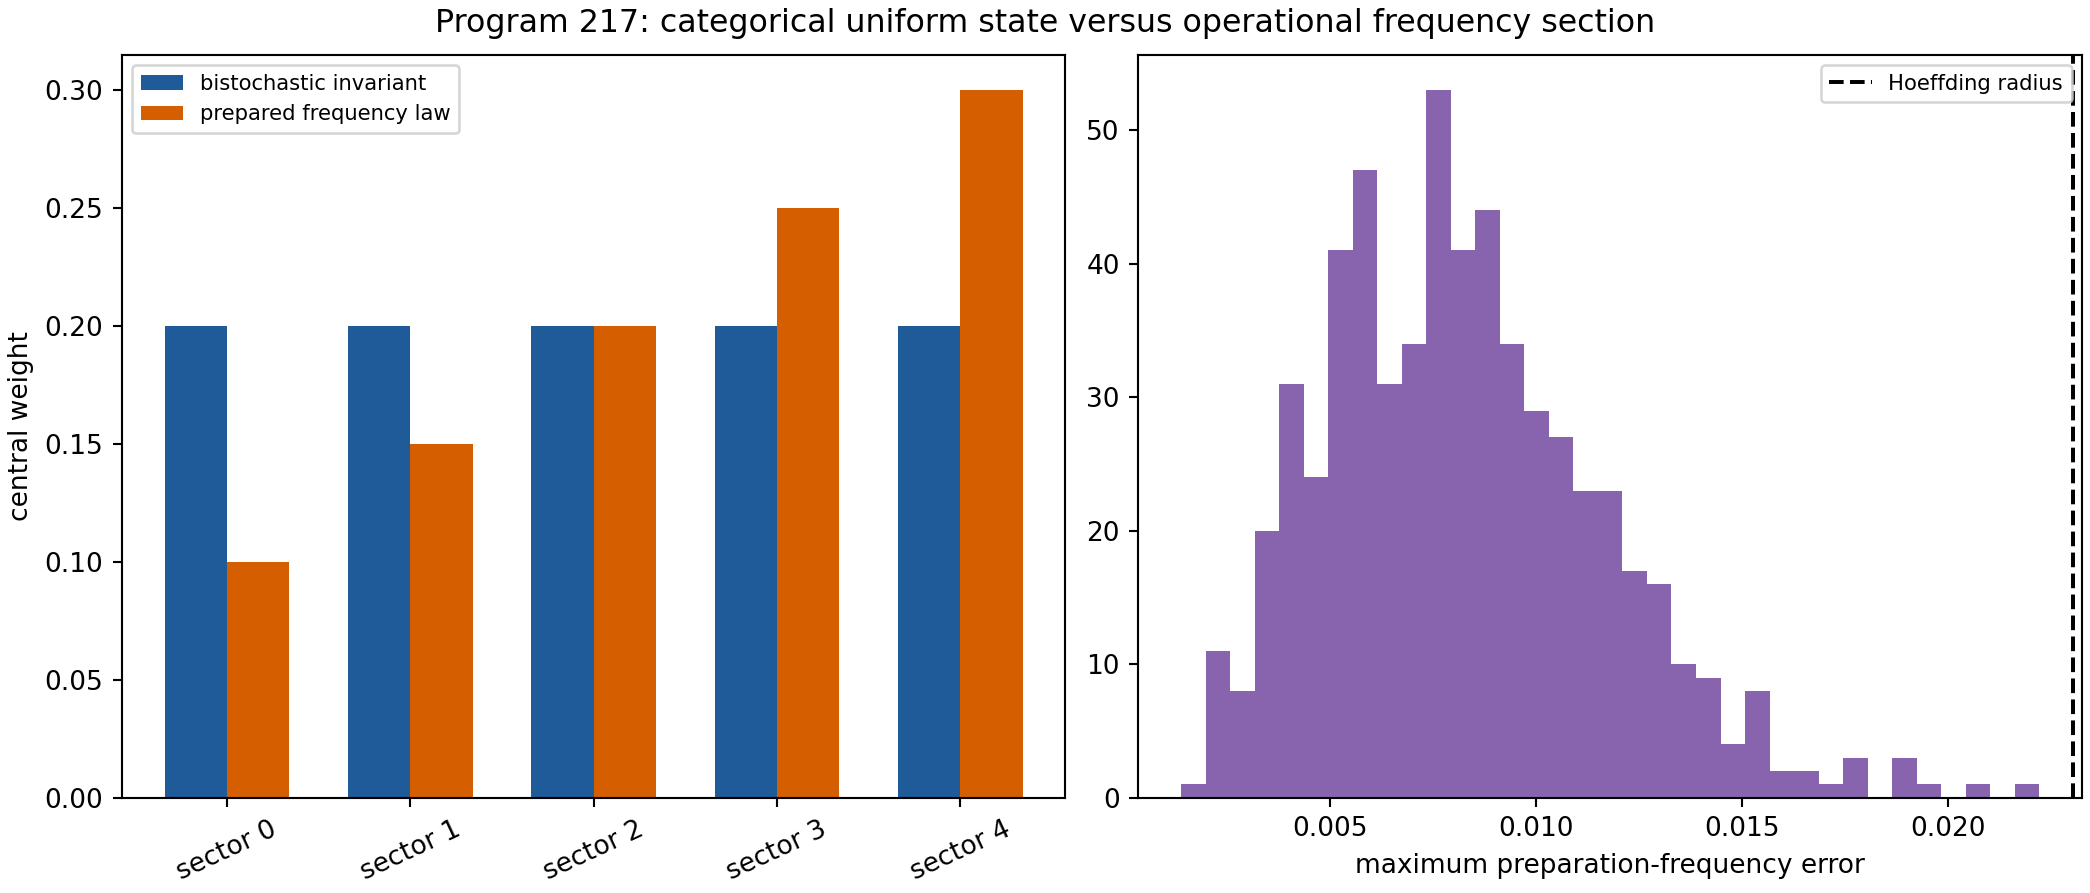
\includegraphics[width=0.94\textwidth]{FIN_Programs_217_229_Operational_Section_Spectral_Tomography_Figures/program217_operational_central_state.png}
\caption{Bistochastic naturality selects the uniform central state, while a preparation record can select and estimate a different state.}
\end{figure}

\par\medskip\hrule\medskip

\chapter{Program 218 --- Affine-natural exponent-flow no-go}

Write the exponent increment as

\[
x=\eta-1.
\]

Suppose its autonomous vector field is natural under changes of positive scale on the increment line:

\[
F(ax)=aF(x)
\qquad
(a>0),
\]

and compatible with reflection:

\[
F(-x)=-F(x).
\]

For \(x>0\),

\[
F(x)=xF(1).
\]

Oddness extends this to every \(x\), so

\[
F(x)=\kappa x.
\]

If \(\kappa\ne0\), the fixed-point equation \(F(x)=0\) has only \(x=0\). If \(\kappa=0\), every \(x\) is fixed. Neither case uniquely selects

\[
x_*=\frac45.
\]

For a polynomial

\[
F(x)=\sum_{j=0}^8c_jx^j,
\]

the single identity \(F(2x)=2F(x)\) gives

\[
(2^j-2)c_j=0.
\]

The coefficient constraint has rank eight, nullity one, and leaves only \(j=1\).

\textbf{Verdict --- Proven.} An offset, non-affine invariant, or other new scale-bearing object is necessary. A target-coded potential with minimum at \(4/5\) is not a source theorem.

\begin{figure}[htbp]
\centering
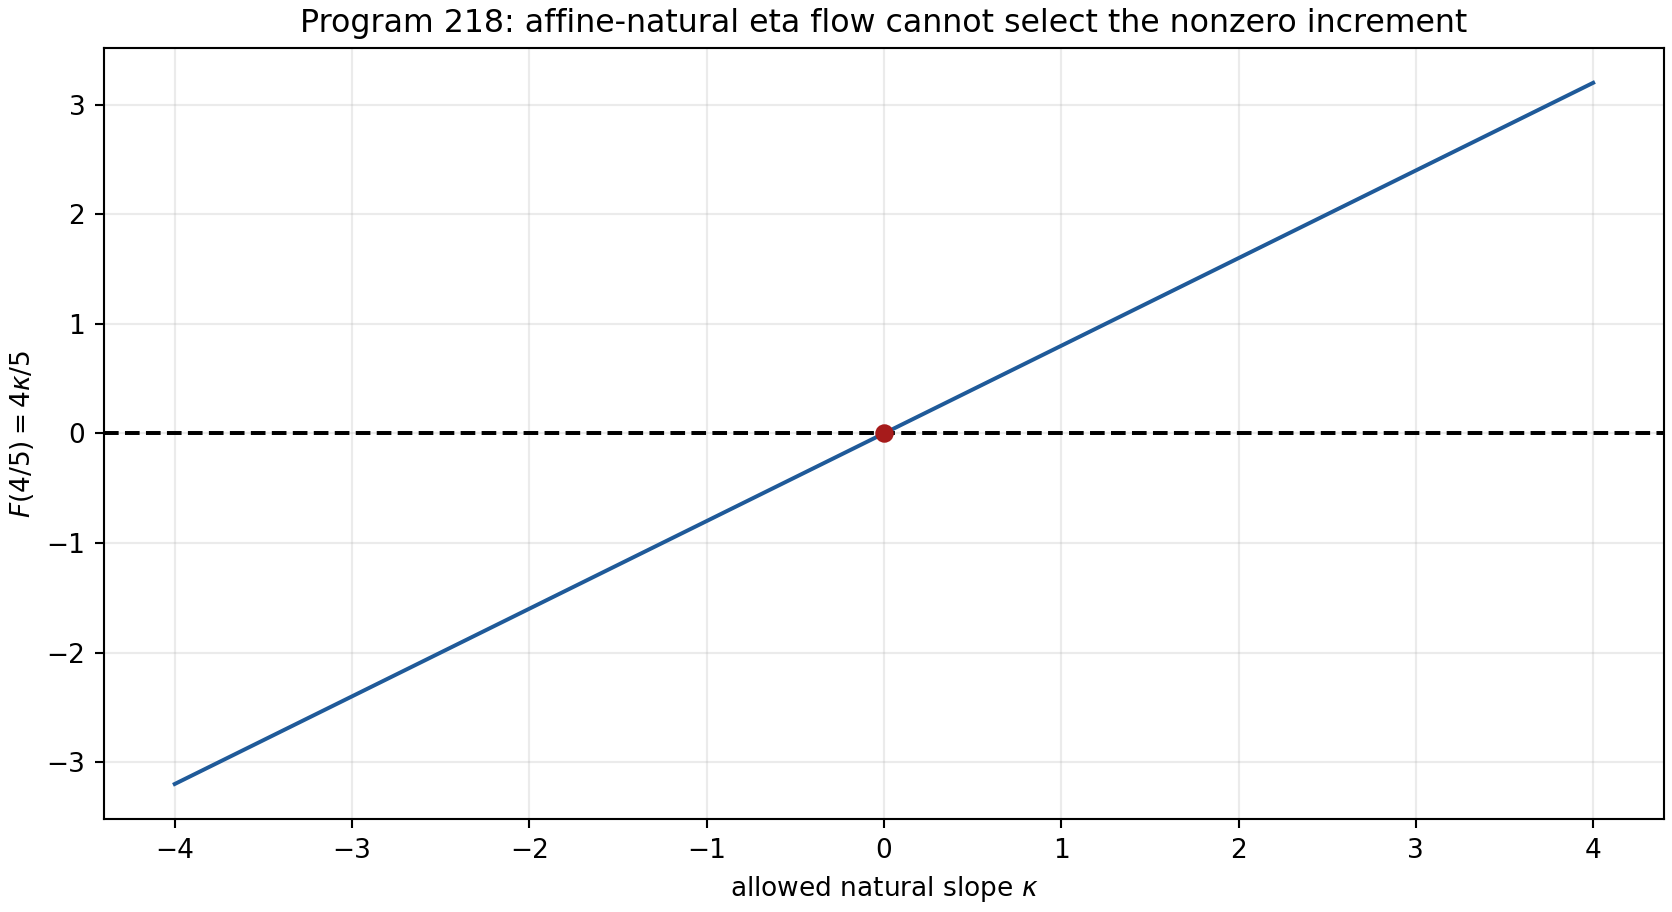
\includegraphics[width=0.94\textwidth]{FIN_Programs_217_229_Operational_Section_Spectral_Tomography_Figures/program218_affine_eta_no_go.png}
\caption{Every allowed affine-natural flow has \(F(4/5)=4\kappa/5\); only the zero flow fixes the target and then fixes every point.}
\end{figure}

\par\medskip\hrule\medskip

\chapter{Program 219 --- Formal Arb execution attestation}

The frozen five-node contract requires one directed-rounding Arb/\allowbreak{}FLINT engine for:

\begin{enumerate}
\item 
finite FFT cells;

\item 
the average/\allowbreak{}polylogarithmic term;

\item 
the cancellation correction tail;

\item 
denominator replacement;

\item 
resonant interval fallbacks.

\end{enumerate}

The current execution probe finds:

\begin{itemize}
\item 
python-flint: absent;

\item 
an arb executable: absent;

\item 
Docker client: present;

\item 
Docker server: inaccessible;

\item 
all-five-node run: not executed;

\item 
sub-three-percent certificate: false.

\end{itemize}

The release adds an immutable attestation referencing the earlier contract hash. It does not download a dependency or replace interval arithmetic with ordinary floating point.

\textbf{Verdict --- Open infrastructure.} This is neither a successful certificate nor a proof that a successful certificate is impossible.

\begin{figure}[htbp]
\centering
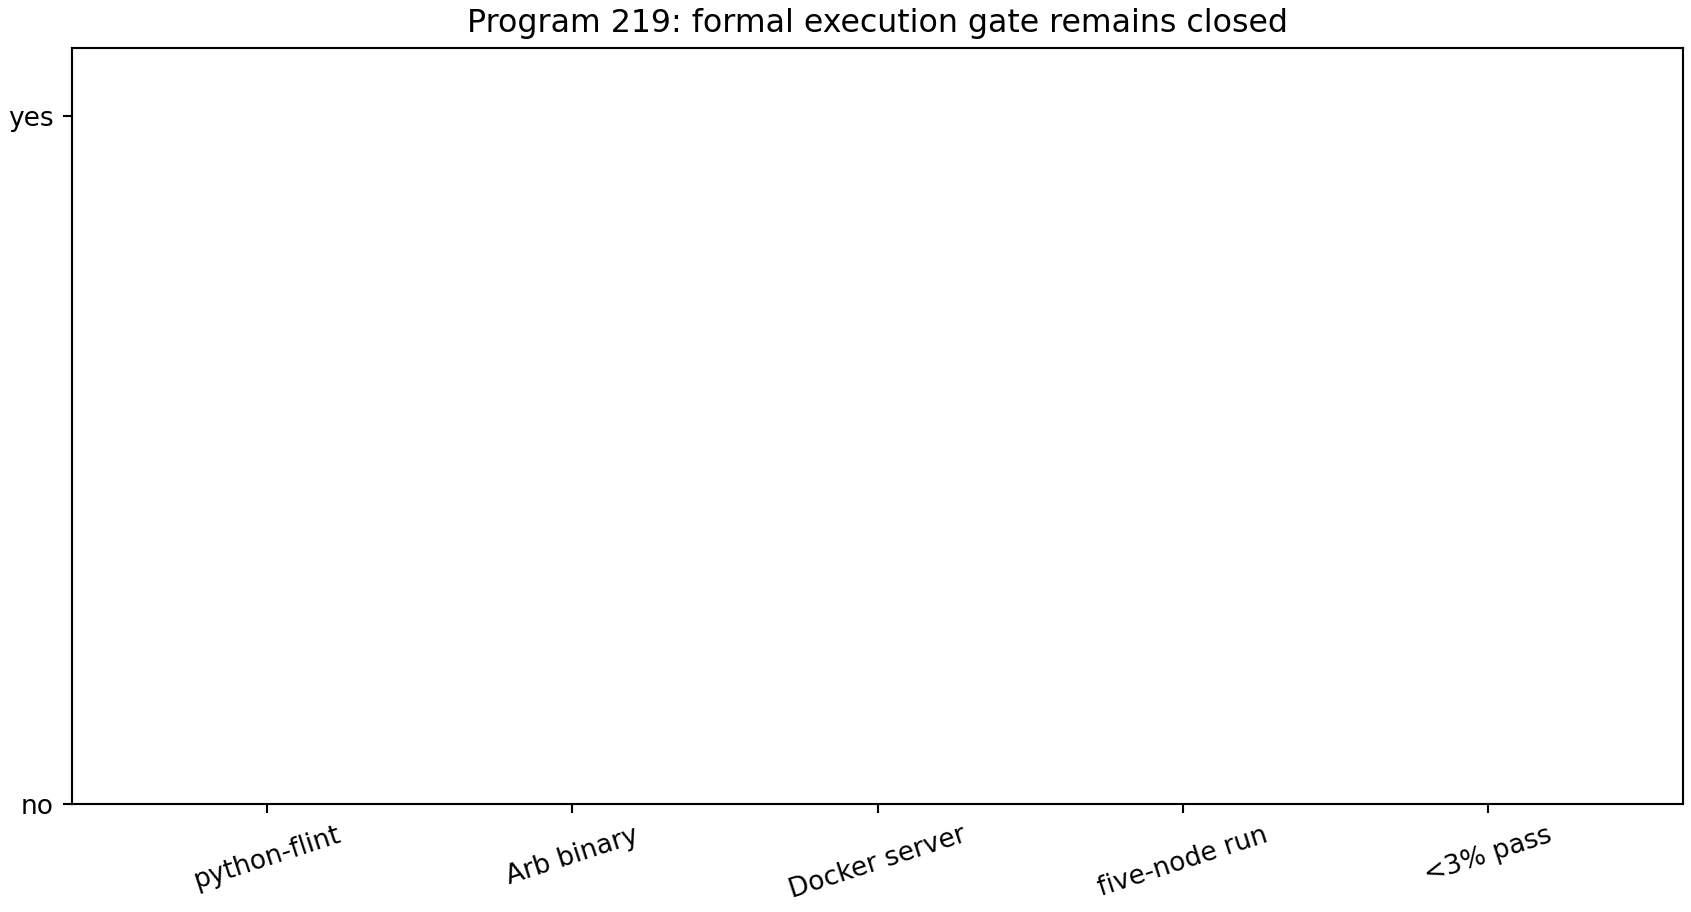
\includegraphics[width=0.94\textwidth]{FIN_Programs_217_229_Operational_Section_Spectral_Tomography_Figures/program219_arb_execution.png}
\caption{The immutable formal execution gate remains closed because no locally callable Arb/FLINT engine is available.}
\end{figure}

\par\medskip\hrule\medskip

\chapter{Program 220 --- Scoped Lean Dirichlet closure}

\section{Compiled finite source}

The new dependency-free Lean source defines two independent integer formulas on the four-cycle:

\[
E_{\rm edge}
=
\sum_{\{i,j\}\in C_4}(x_i-x_j)^2,
\]

and

\[
E_{\rm Lap}
=
2\sum_i x_i^2
-2\sum_{\{i,j\}\in C_4}x_ix_j.
\]

Lean machine-checks:

\begin{itemize}
\item 
the constant null mode for both formulas;

\item 
equality of the two formulas on the archived vector \((1,2,-1,3)\);

\item 
exact energy \(30\);

\item 
nonnegativity of that energy.

\end{itemize}

The compiler outputs 30 and exits with status zero.

\section{General library boundary}

The general source still imports Mathlib matrix, positivity, and complex exponential modules. Compilation stops at

unknown module prefix 'Mathlib'

before theorem checking.

\textbf{Verdict --- Machine checked in stated finite scope.} The concrete formal certificate is real. The general weighted-graph Dirichlet theorem and heat semigroup remain analytic, not proof-assistant-closed.

\begin{figure}[htbp]
\centering
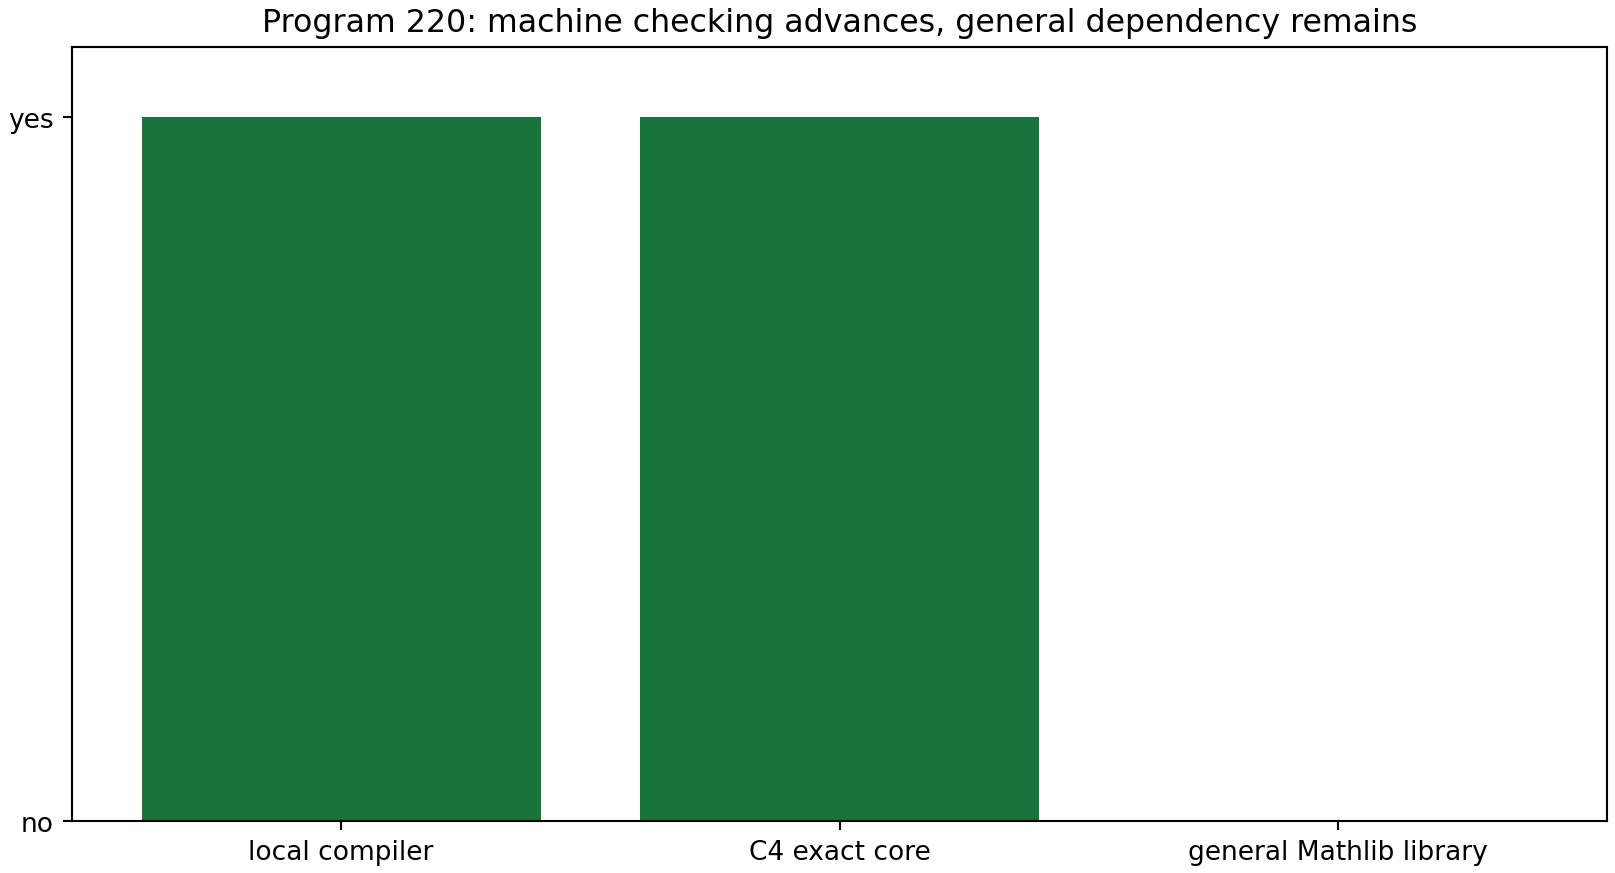
\includegraphics[width=0.94\textwidth]{FIN_Programs_217_229_Operational_Section_Spectral_Tomography_Figures/program220_lean_build.png}
\caption{The dependency-free four-cycle certificate compiles; the general Mathlib graph library remains dependency-blocked.}
\end{figure}

\par\medskip\hrule\medskip

\chapter{Program 221 --- Cost of an imperfect symmetry reference}

\section{Product-return no-broadcast theorem}

Let reflection exchange

\[
\kappa_r^\pm=\frac{I\pm r\sigma_x}{2}.
\]

Their squared Uhlmann fidelity is

\[
\mathcal F(\kappa_r^+,\kappa_r^-)=1-r^2.
\]

Suppose no second asymmetric input is consumed and a covariant channel is required to produce a target orbit \(\tau_t^\pm\) while returning the reference exactly and without correlation:

\[
\kappa_r^\pm
\longmapsto
\tau_t^\pm\otimes\kappa_r^\pm.
\]

For a transverse target of magnitude \(t\),

\[
\mathcal F(\tau_t^+,\tau_t^-)=1-t^2.
\]

Fidelity is multiplicative on products, hence the output fidelity is

\[
(1-r^2)(1-t^2).
\]

A channel cannot decrease fidelity. For \(r<1\) and \(t>0\),

\[
(1-r^2)(1-t^2)<1-r^2,
\]

a contradiction.

The perfect reference \(r=1\) lies exactly on the zero-fidelity boundary and is not excluded, consistently with Program 208.

\section{Correlated marginal return}

Measure the imperfect reference in the \(\sigma_x\) basis. Conditional on \(X=\pm1\), prepare a system state with transverse coordinate \(\pm q\). The nonselective reference marginal remains \(\kappa_r\), while the system marginal has coordinate

\[
t=rq.
\]

Thus any \(t\le r\) is reachable with \(q=t/r\), but the system and reference are correlated.

For \(r=0.8\) and \(t=0.6\),

\[
q=0.75,
\qquad
I(X:Y)=0.1783636517\ {\rm bits}.
\]

The missing resource has become measurable: exact marginal reuse stores a correlation ledger.

\section{Boundary}

The theorem does not classify a conversion in which another asymmetric source is consumed. It also does not derive the reference sign. It proves that imperfect orientation cannot be freely broadcast in product form.

\textbf{Verdict --- Proven.} A perfect reference, source consumption, disturbance, approximation, or accumulated correlation is necessary.

\begin{figure}[htbp]
\centering
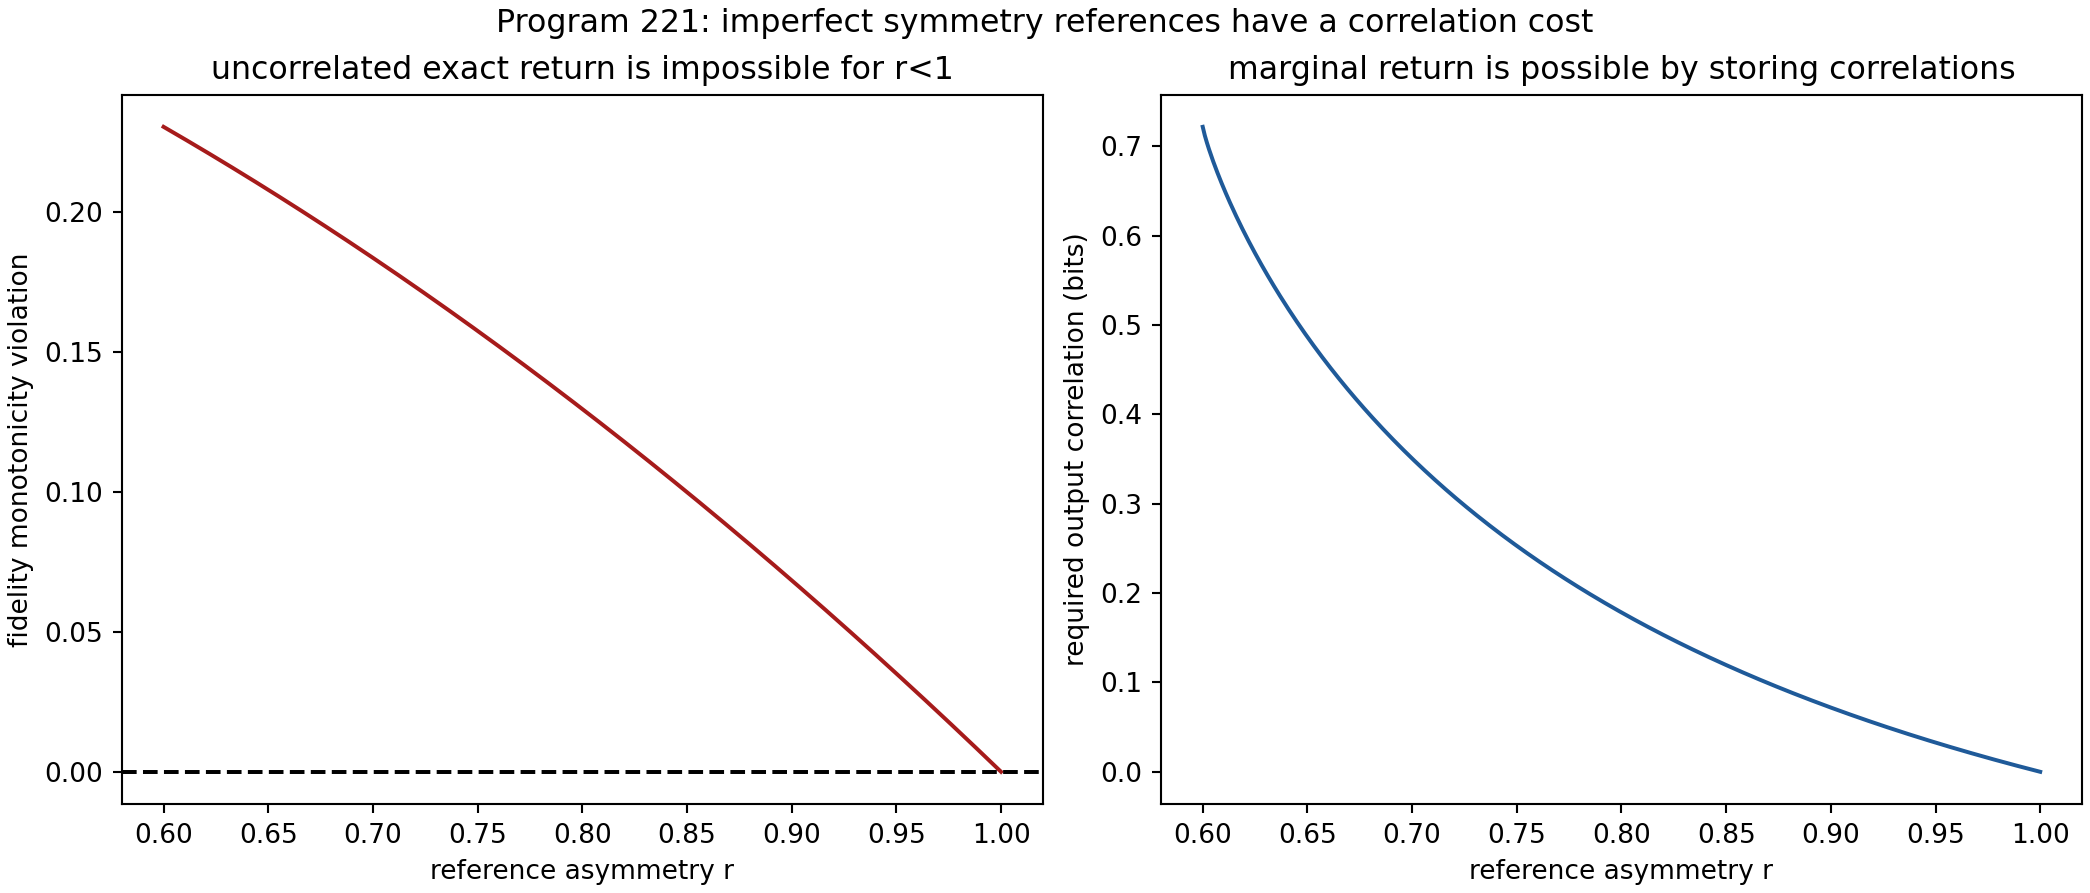
\includegraphics[width=0.94\textwidth]{FIN_Programs_217_229_Operational_Section_Spectral_Tomography_Figures/program221_reference_cost.png}
\caption{Imperfect product return violates fidelity monotonicity, whereas marginal return stores a measurable target--reference correlation.}
\end{figure}

\par\medskip\hrule\medskip

\chapter{Program 222 --- Optimal hidden-mixing acquisition}

Assume the target record satisfies

\[
\beta(k)\le(1-p_0)^k
\]

but \(p_0\) is learned from a separate calibration experiment.

For thinning lag \(L\) and retained count \(m\), allocate a per-sequence failure budget \(\delta_s\) between

\[
\delta_{\rm coupling}
=(m-1)(1-p_0)^L
\]

and

\[
\delta_{\rm DKW}
=
\delta_s-\delta_{\rm coupling}.
\]

The DKW radius is

\[
\varepsilon(L)
=
\sqrt{
\frac{\log(2/\delta_{\rm DKW})}{2m}
}.
\]

Program 222 minimizes this expression over every integer \(L\).

In a calibration of 10,000 trials with 608 observed refreshes, the one-sided \(99\%\) lower confidence bound is

\[
\widehat p_0^-=0.0553654.
\]

After allocating \(0.01\) failure probability to calibration and \(0.02\) to each of two target sequences, the robust optimum is

\[
L=161,
\qquad
m=63,
\qquad
\varepsilon=0.199102.
\]

The inherited equal-split design had \(\varepsilon=0.203960\). An oracle using the true \(p=0.06\) reaches \(0.185448\). Across 3,000 calibration simulations, the one-sided lower bound covers in \(0.990333\) of trials.

\textbf{Verdict --- Proven bound and exhaustive finite optimization.} A separate mixing calibration remains an apparatus input.

\begin{figure}[htbp]
\centering
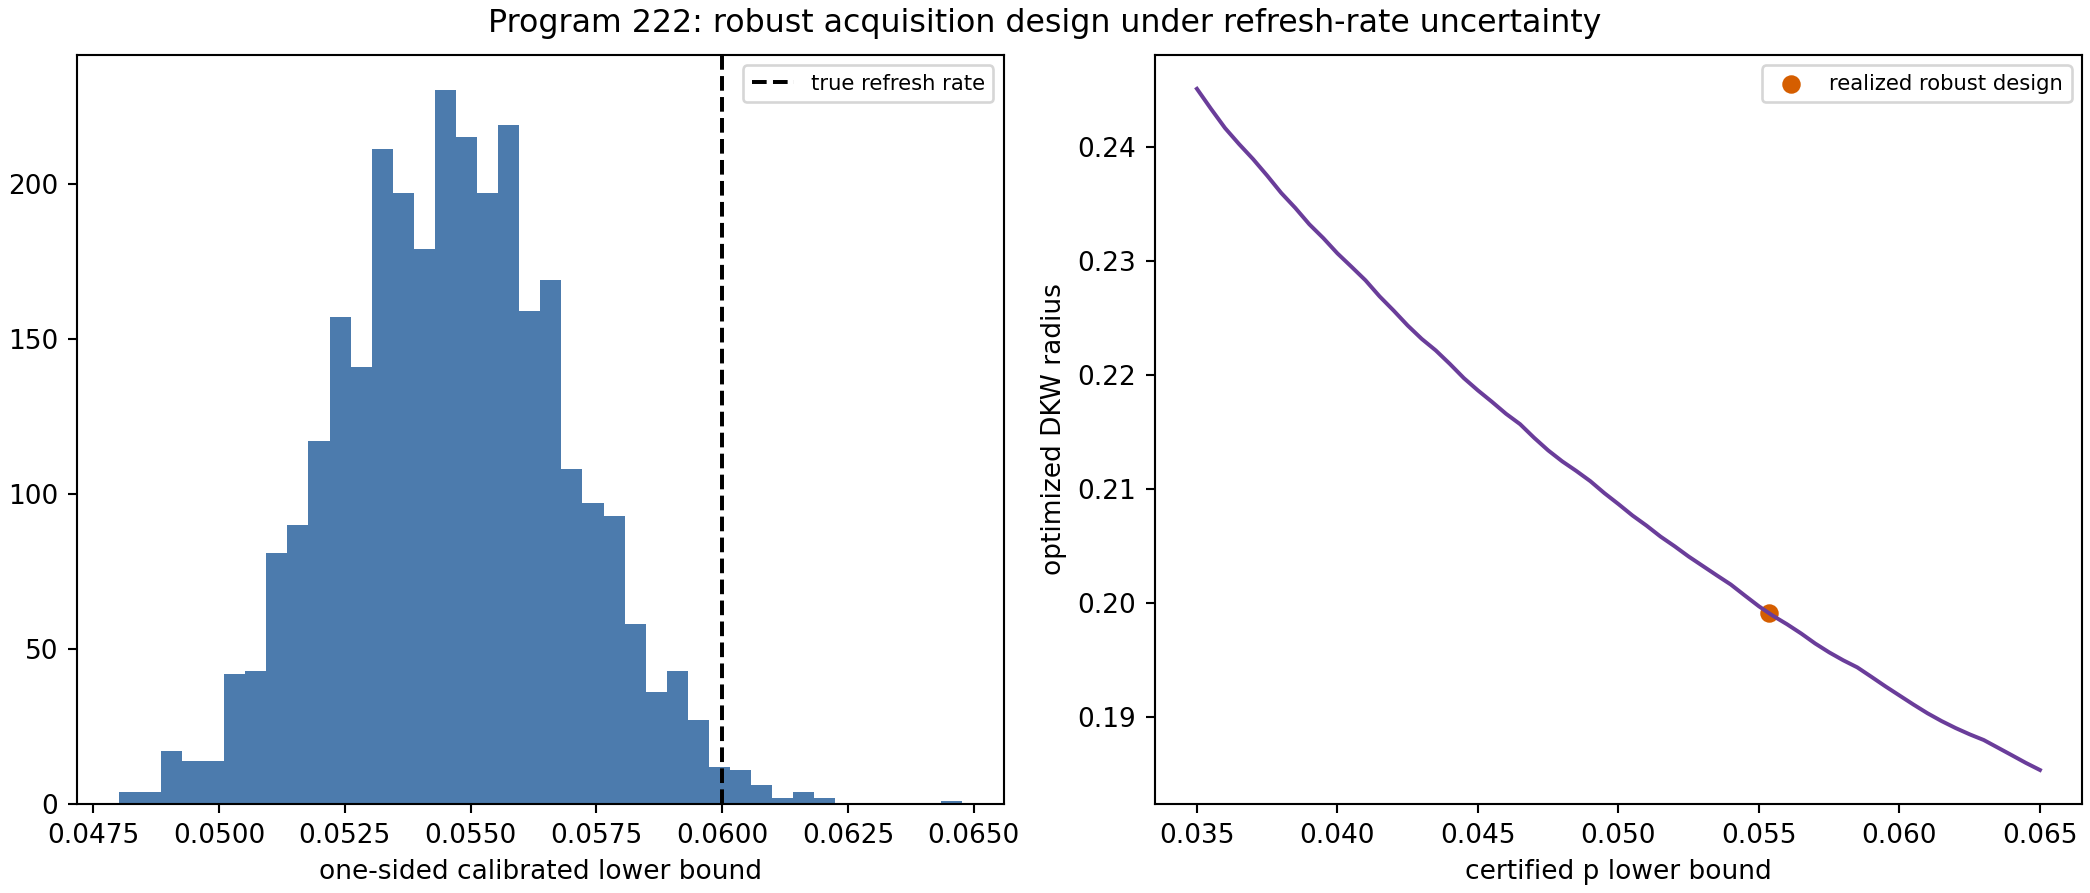
\includegraphics[width=0.94\textwidth]{FIN_Programs_217_229_Operational_Section_Spectral_Tomography_Figures/program222_robust_mixing_design.png}
\caption{A calibrated lower refresh bound and exact budget optimization determine the robust thinning design.}
\end{figure}

\par\medskip\hrule\medskip

\chapter{Program 223 --- Reusable-calibration insertion-rank e-process}

\section{Construction}

For iid continuous scores \(S_1,S_2,\ldots\), let \(R_N\) be the descending insertion rank of \(S_N\) among \(S_1,\ldots,S_N\). The sequential insertion ranks are independent, with

\[
R_N\sim\operatorname{Uniform}\{1,\ldots,N\}.
\]

Define

\[
e_N=\frac{N}{H_NR_N},
\qquad
H_N=\sum_{r=1}^N\frac1r.
\]

Then

\[
\mathbb E[e_N]=1,
\]

and

\[
E_n=\prod_{N=m+1}^{m+n}e_N
\]

is a nonnegative mean-one martingale in the filtration generated by the insertion ranks. Ville's bound applies to stopping rules measurable in that filtration.

\section{Challenge}

With 30 initial records, horizon 50, and 1,200 streams:

\begin{itemize}
\item 
iid-null rejection is \(0.029167\) at threshold \(20\);

\item 
the shifted alternative rejects in every trial;

\item 
mean alternative crossing time is \(2.51083\).

\end{itemize}

\section{Why naive fixed reuse is not the theorem}

If every future score is ranked only against one fixed calibration block, the one-step e-value need not have conditional mean at most one after the actual calibration values are revealed. Across 5,000 calibration samples, more than one quarter have conditional mean above one, and the maximum observed conditional mean exceeds \(1.5\).

The insertion-rank construction repairs this by updating the pool and using the rank filtration. It does not establish validity for arbitrary stopping rules using the raw score values.

\textbf{Verdict --- Proven in the declared filtration; strong synthetic power.}

\begin{figure}[htbp]
\centering
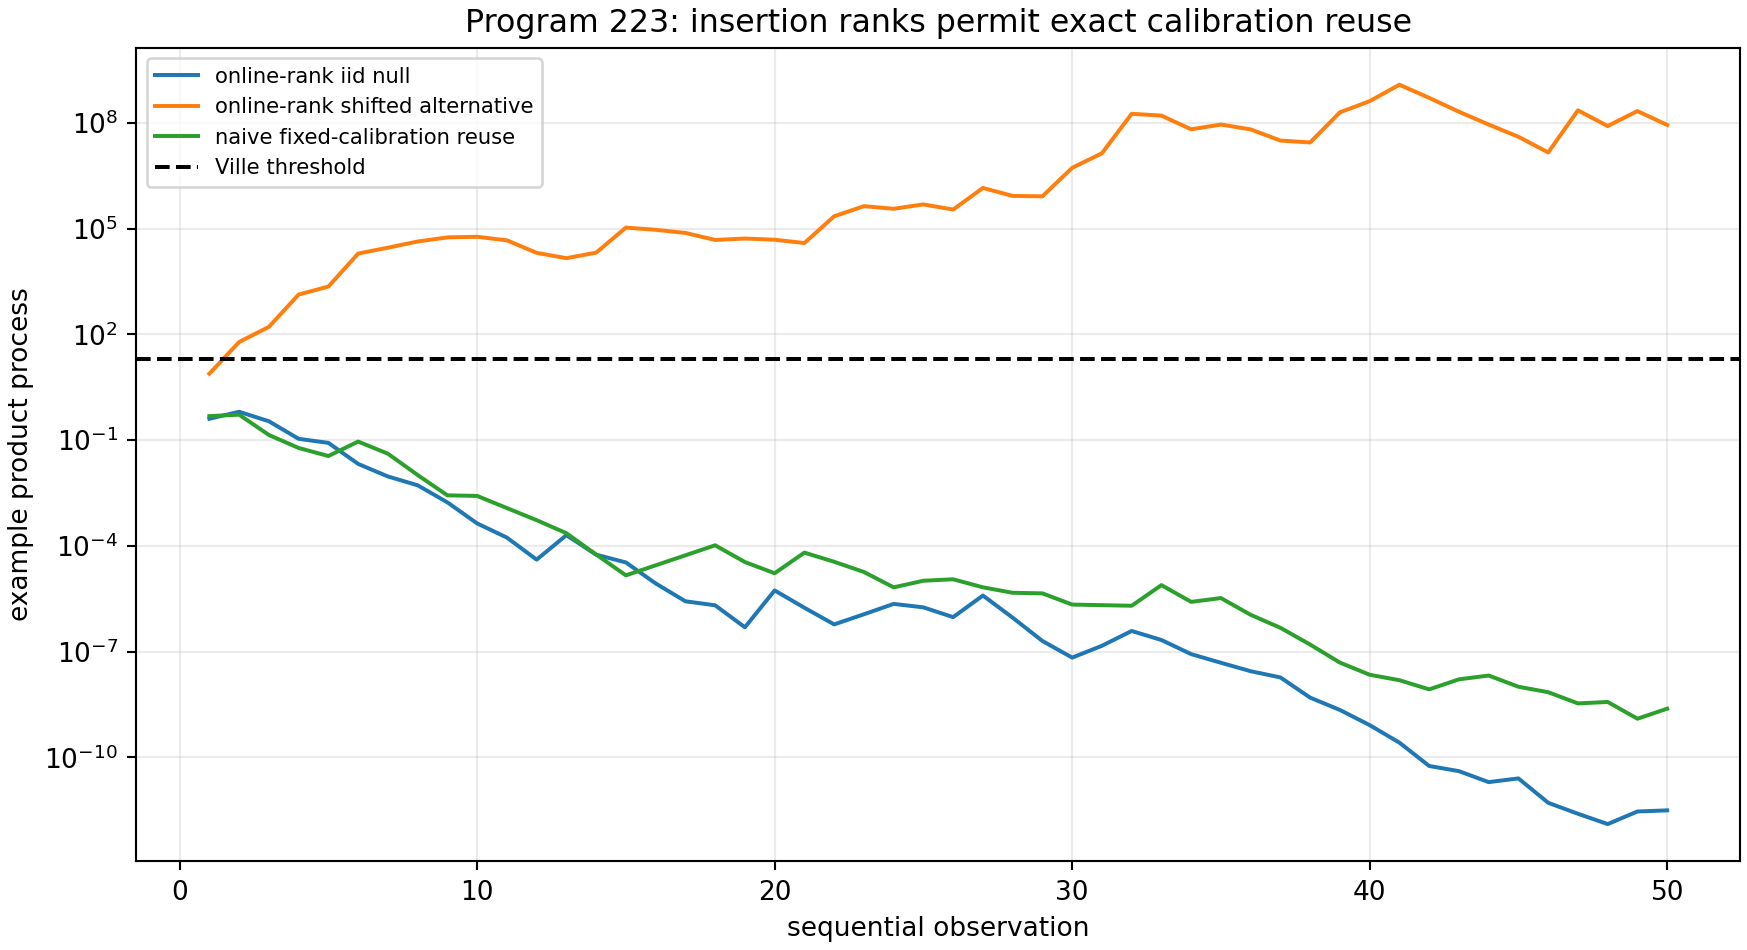
\includegraphics[width=0.94\textwidth]{FIN_Programs_217_229_Operational_Section_Spectral_Tomography_Figures/program223_reusable_eprocess.png}
\caption{Sequential insertion ranks support an anytime-valid rank-filtration e-process while fixed calibration reuse lacks the same conditional law.}
\end{figure}

\par\medskip\hrule\medskip

\chapter{Program 224 --- Efficient process regions and misspecification}

\section{Log-linear estimator}

For the three visibilities

\[
V_1=be^{-v/2},
\qquad
V_+=be^{-v-c},
\qquad
V_-=be^{-v+c},
\]

write \(\ell=(\log V_1,\log V_+,\log V_-)^\mathsf T\). Then

\[
\begin{pmatrix}
\log b\\
v\\
c
\end{pmatrix}
=
\begin{pmatrix}
2&-1/2&-1/2\\
2&-1&-1\\
0&-1/2&1/2
\end{pmatrix}
\ell.
\]

The covariance is propagated from six independent binomial counts. A \(95\%\) likelihood-quadratic ellipsoid uses the \(\chi^2_3\) radius.

\section{Results}

At 1,000 shots per phase/\allowbreak{}context and 1,200 simulations:

\begin{itemize}
\item 
simultaneous empirical coverage: \(0.956667\);

\item 
memory-detection power: \(1.0\);

\item 
mean widths for \((\log b,v,c)\): \((0.313519,0.404383,0.147349)\).

\end{itemize}

The corresponding exact conservative Program-211 widths were

\[
(0.652869,0.928039,0.275169).
\]

\section{Independent model control}

An independent fourth contrast tests

\[
\log V_4=\log b-2v.
\]

Its null rejection rate is \(0.040833\). Multiplying the true contrast by \(e^{-0.20}\) raises rejection to \(0.408333\).

\section{Claim boundary}

The width reduction is purchased by asymptotics. The ellipsoid is not an exact finite-sample confidence set. Program 211 remains the rigorous conservative option; Program 224 is an efficient, falsifiable approximation.

\textbf{Verdict --- Strong evidence, not a finite-sample theorem.}

\begin{figure}[htbp]
\centering
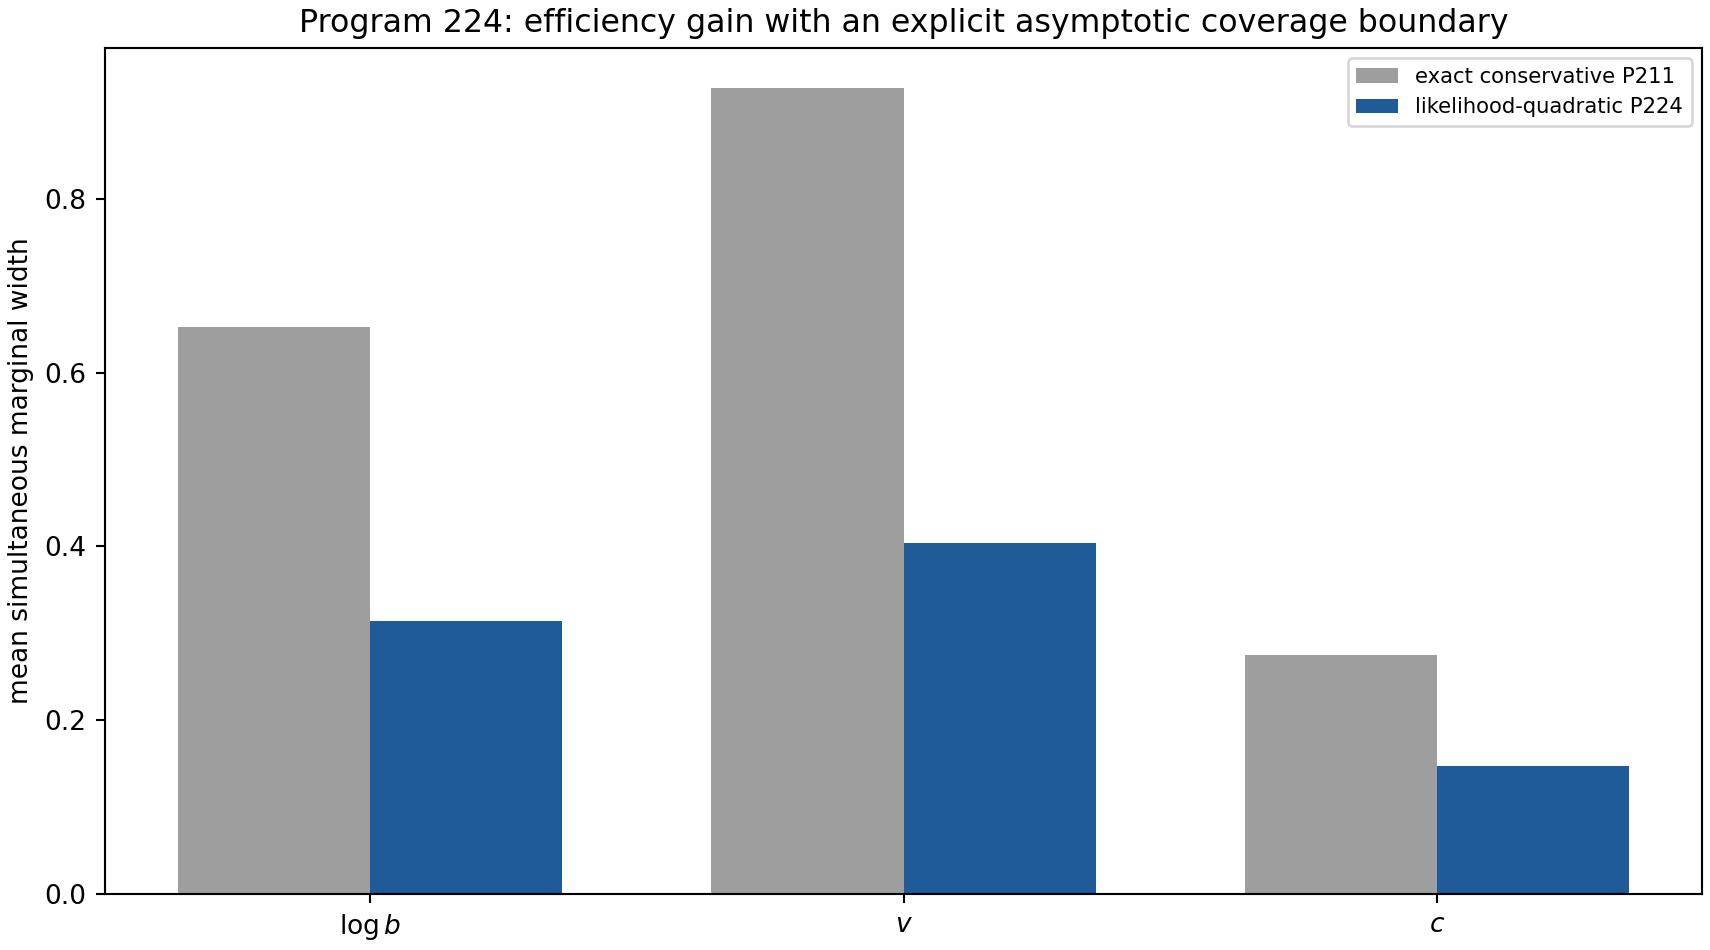
\includegraphics[width=0.94\textwidth]{FIN_Programs_217_229_Operational_Section_Spectral_Tomography_Figures/program224_likelihood_region.png}
\caption{The likelihood-quadratic region is substantially narrower than the exact conservative region, with its asymptotic boundary kept explicit.}
\end{figure}

\par\medskip\hrule\medskip

\chapter{Program 225 --- Sharp third environmental moment}

Let

\[
c_k=\int\cos(k\theta)\,d\mu(\theta)
\]

for a real symmetric probability measure on the circle. Given

\[
c_1=\frac45,
\qquad
c_2=\frac12,
\]

the order-three Toeplitz matrix is

\[
T_3=
\begin{pmatrix}
1&c_1&c_2&c_3\\
c_1&1&c_1&c_2\\
c_2&c_1&1&c_1\\
c_3&c_2&c_1&1
\end{pmatrix}.
\]

The leading \(T_2\) block is positive definite and

\[
\det T_3
=
-\frac{(20c_3-11)(180c_3+11)}{10000}.
\]

Therefore

\[
-\frac{11}{180}
\le c_3\le
\frac{11}{20}.
\]

Since the leading block is positive definite, the determinant condition is equivalent to the final scalar Schur-complement condition.

\section{Lower extremizer}

In \(x=\cos\theta\), place mass \(11/335\) at \(x=-1\) and mass \(324/335\) at \(x=31/36\). Symmetrically on the circle this is:

\begin{itemize}
\item 
mass \(11/335\) at \(\theta=\pi\);

\item 
mass \(162/335\) at each of \(\theta=\pm\arccos(31/36)\).

\end{itemize}

Its first three ordinary \(x\) moments are

\[
\left(
\frac45,\frac34,\frac{421}{720}
\right),
\]

and \(4E[x^3]-3E[x]=-11/180\).

\section{Upper extremizer}

Place mass \(11/15\) at \(x=1\) and mass \(4/15\) at \(x=1/4\). On the circle:

\begin{itemize}
\item 
mass \(11/15\) at \(\theta=0\);

\item 
mass \(2/15\) at each of \(\theta=\pm\arccos(1/4)\).

\end{itemize}

The ordinary moments are

\[
\left(
\frac45,\frac34,\frac{59}{80}
\right),
\]

and \(4E[x^3]-3E[x]=11/20\).

\textbf{Verdict --- Proven and sharp.} The environment remains nonunique throughout the interval.

\begin{figure}[htbp]
\centering
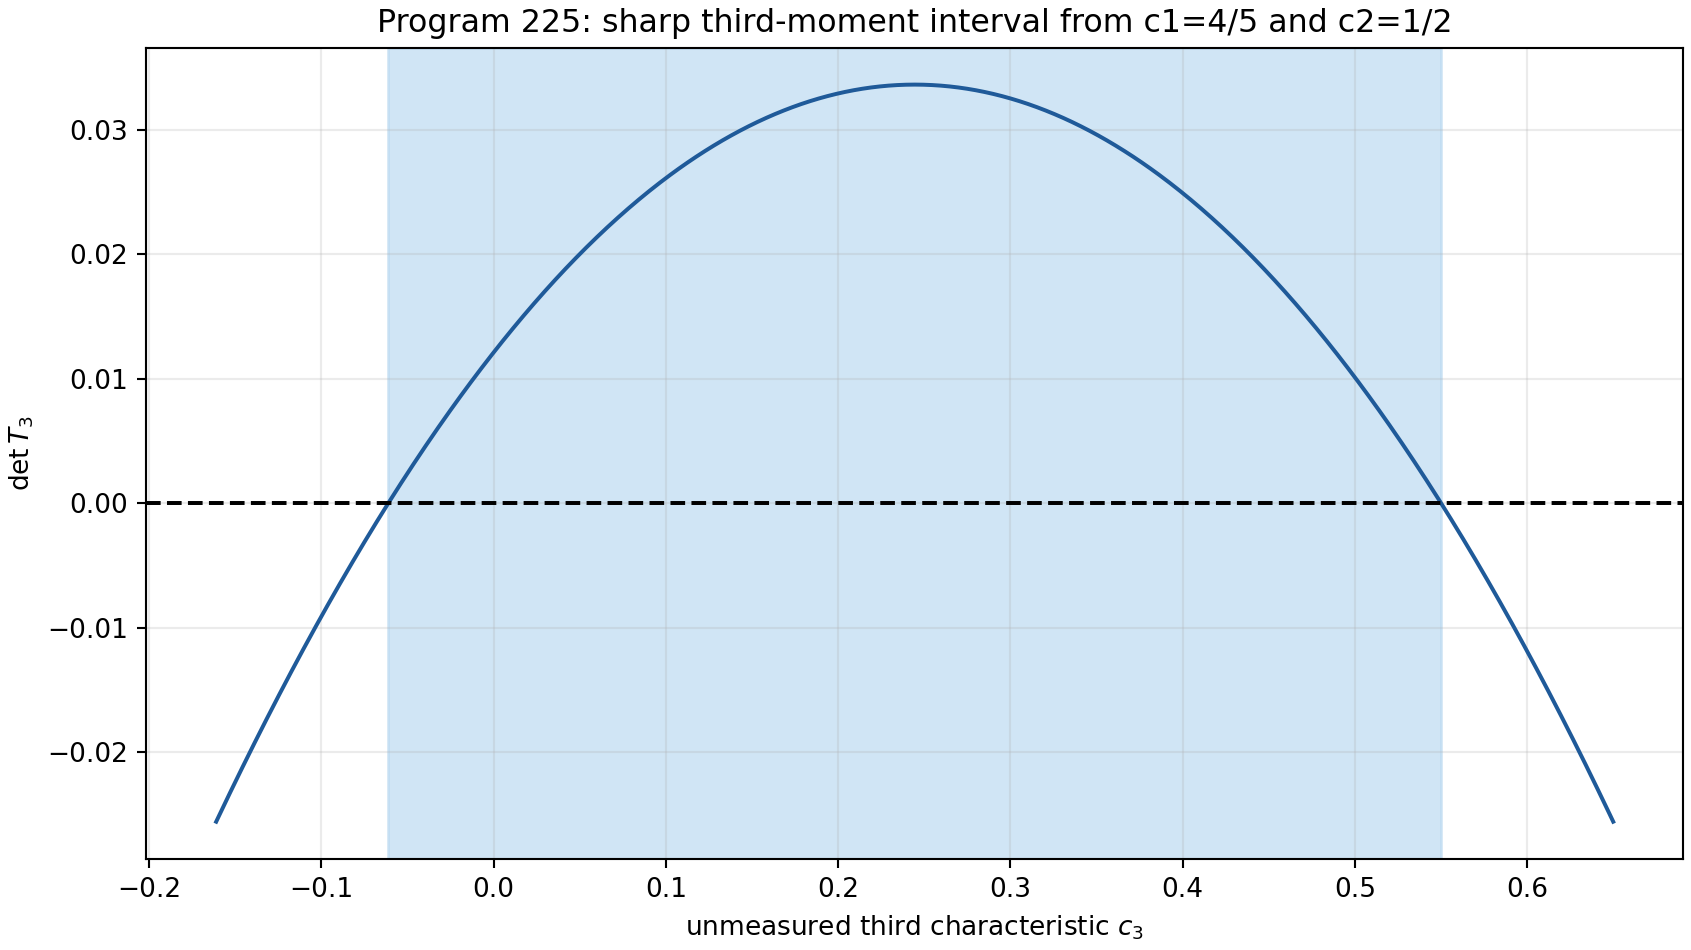
\includegraphics[width=0.94\textwidth]{FIN_Programs_217_229_Operational_Section_Spectral_Tomography_Figures/program225_higher_moment.png}
\caption{Toeplitz positivity gives the sharp interval \(-11/180\le c_3\le11/20\).}
\end{figure}

\par\medskip\hrule\medskip

\chapter{Program 226 --- Scoped formal phase certificate}

The dependency-free Lean source machine-checks:

\[
\{n\bmod8:n=0,\ldots,7\}
=
\{0,\ldots,7\},
\]

that every image remains an order-eight residue slot, and

\[
\gcd(743,4000)=1.
\]

It does not machine-check:

\begin{itemize}
\item 
the classification \(h(z)=z^n\) of continuous \(U(1)\) endomorphisms;

\item 
automatic continuity of Borel homomorphisms;

\item 
the transcendence argument proving \(e^{i743/4000}\) is non-torsion.

\end{itemize}

Those remain analytic mathematics inherited from Program 213.

\textbf{Verdict --- Finite core machine checked; analytic hierarchy open in Lean.} No strict phase source is produced.

\begin{figure}[htbp]
\centering
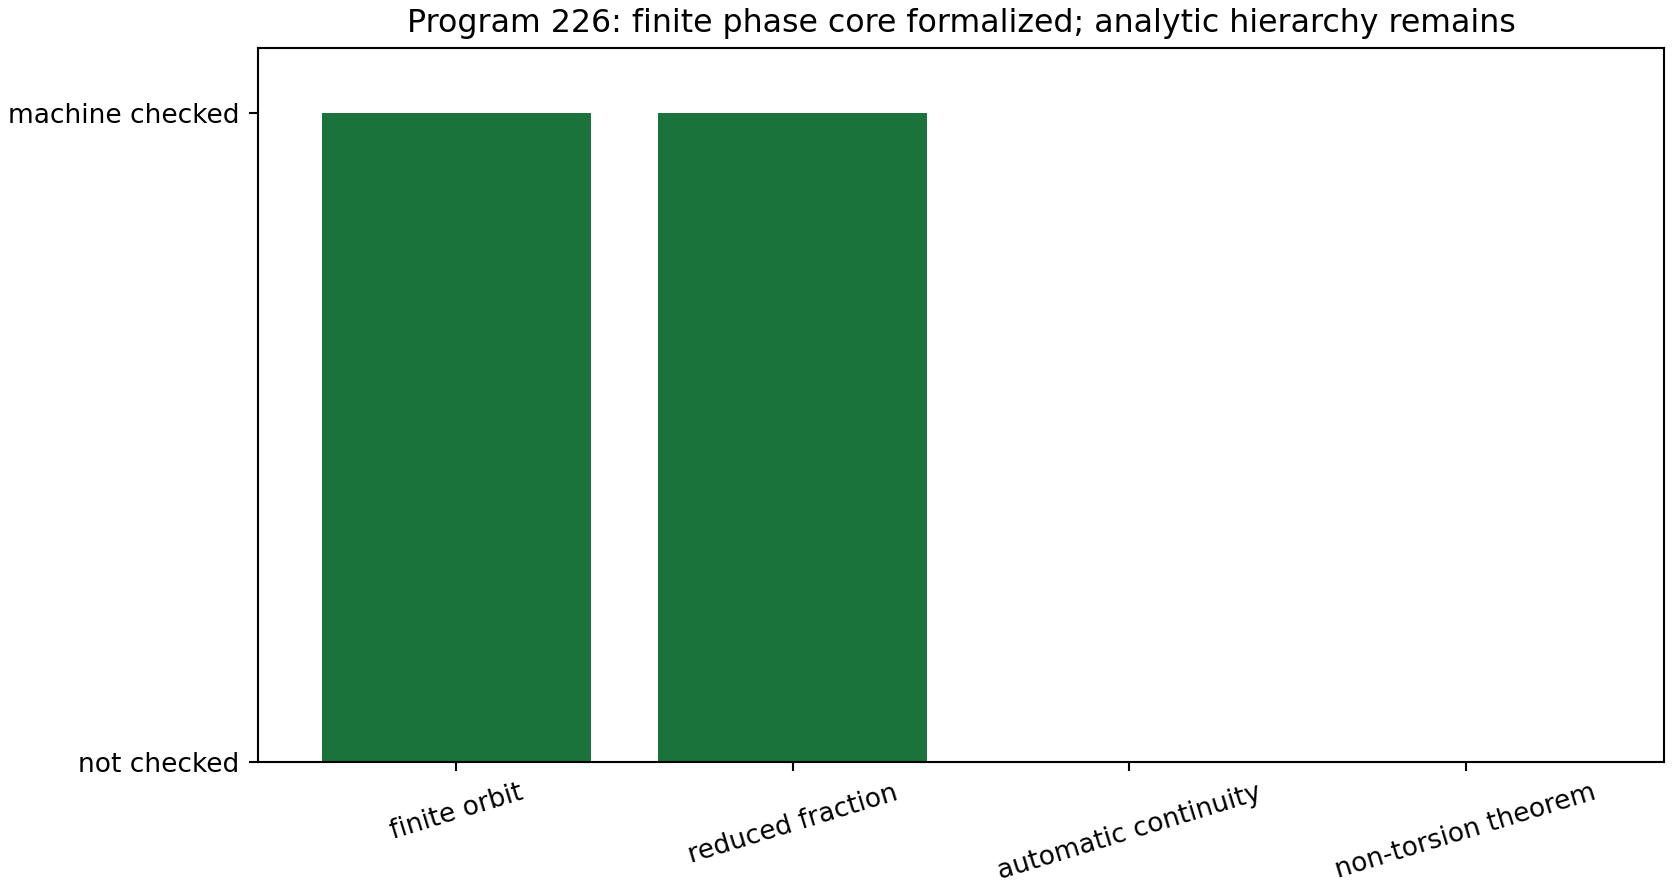
\includegraphics[width=0.94\textwidth]{FIN_Programs_217_229_Operational_Section_Spectral_Tomography_Figures/program226_phase_formalization.png}
\caption{The finite torsion orbit is machine checked; automatic continuity and the transcendence theorem remain analytic.}
\end{figure}

\par\medskip\hrule\medskip

\chapter{Program 227 --- Heat-kernel spectral tomography}

\section{Instrument}

On a twelve-node finite system:

\begin{enumerate}
\item 
prepare each basis state \(e_j\);

\item 
evolve for one positive duration \(\tau\) under \(P_\tau=e^{-\tau A}\);

\item 
measure the twelve-outcome vertex POVM;

\item 
record the conditional probabilities \((P_\tau)_{ij}\).

\end{enumerate}

The full experiment reconstructs one transition matrix column per preparation.

\section{Identifiability theorem}

For symmetric \(A\ge0\), the heat matrix \(P_\tau\) is symmetric positive definite. The exponential is injective on real symmetric matrices after restricting to the principal logarithm:

\[
A=-\frac1\tau\log P_\tau.
\]

If the clock scale is unknown, write the transition eigenvalues as

\[
\mu_k=e^{-\tau\lambda_k}.
\]

Then

\[
\frac{\lambda_k}{\lambda_{\max}}
=
\frac{\log\mu_k}{\log\mu_{\min}}.
\]

Thus the projective signature is identifiable without choosing an absolute energy or time unit.

\section{Stability theorem}

If

\[
\|\widehat P-P\|_2\le\varepsilon
<
\lambda_{\min}(P),
\]

Weyl's theorem bounds every eigenvalue error by \(\varepsilon\). On \([\lambda_{\min}(P)-\varepsilon,1+\varepsilon]\), the logarithm is Lipschitz with constant at most

\[
\frac1{\lambda_{\min}(P)-\varepsilon}.
\]

This gives an explicit error bound for the reconstructed rates and, after normalization away from zero maximum rate, for the projective fingerprint.

\section{Finite-shot challenge}

The simulated duration is

\[
\tau=\lambda_{\max}^{-1}
=
0.4269522959,
\]

so

\[
\lambda_{\min}(P_\tau)=e^{-1}=0.3678794412.
\]

Exact reconstruction has signature residual \(7.77\times10^{-16}\).

\begin{center}
\begingroup\small
\setlength{\tabcolsep}{3.5pt}
\renewcommand{\arraystretch}{1.16}
\begin{longtable}{@{}p{0.274\textwidth}p{0.193\textwidth}p{0.237\textwidth}p{0.157\textwidth}@{}}
\toprule
\textbf{Shots per preparation} & \textbf{Mean distance} & \textbf{95th percentile} & \textbf{P214 pass rate} \\
\midrule
\endhead
2,000 & 0.044333 & 0.072210 & 0.0375 \\
10,000 & 0.016112 & 0.024442 & 0.7292 \\
50,000 & 0.006215 & 0.009920 & 1.0000 \\
\bottomrule
\end{longtable}
\endgroup
\end{center}

The low-shot failure rate is scientifically important: the protocol does not declare finite precision sufficient merely because the model is exact.

\section{Physical boundary}

The construction proves an instrument theorem. It does not prove that a laboratory realizes the twelve basis states, the vertex POVM, or a time-homogeneous FIN semigroup. Those belong to the operational and external data layers.

\textbf{Verdict --- Proven identifiability and stability; strong finite-shot evidence.}

\begin{figure}[htbp]
\centering
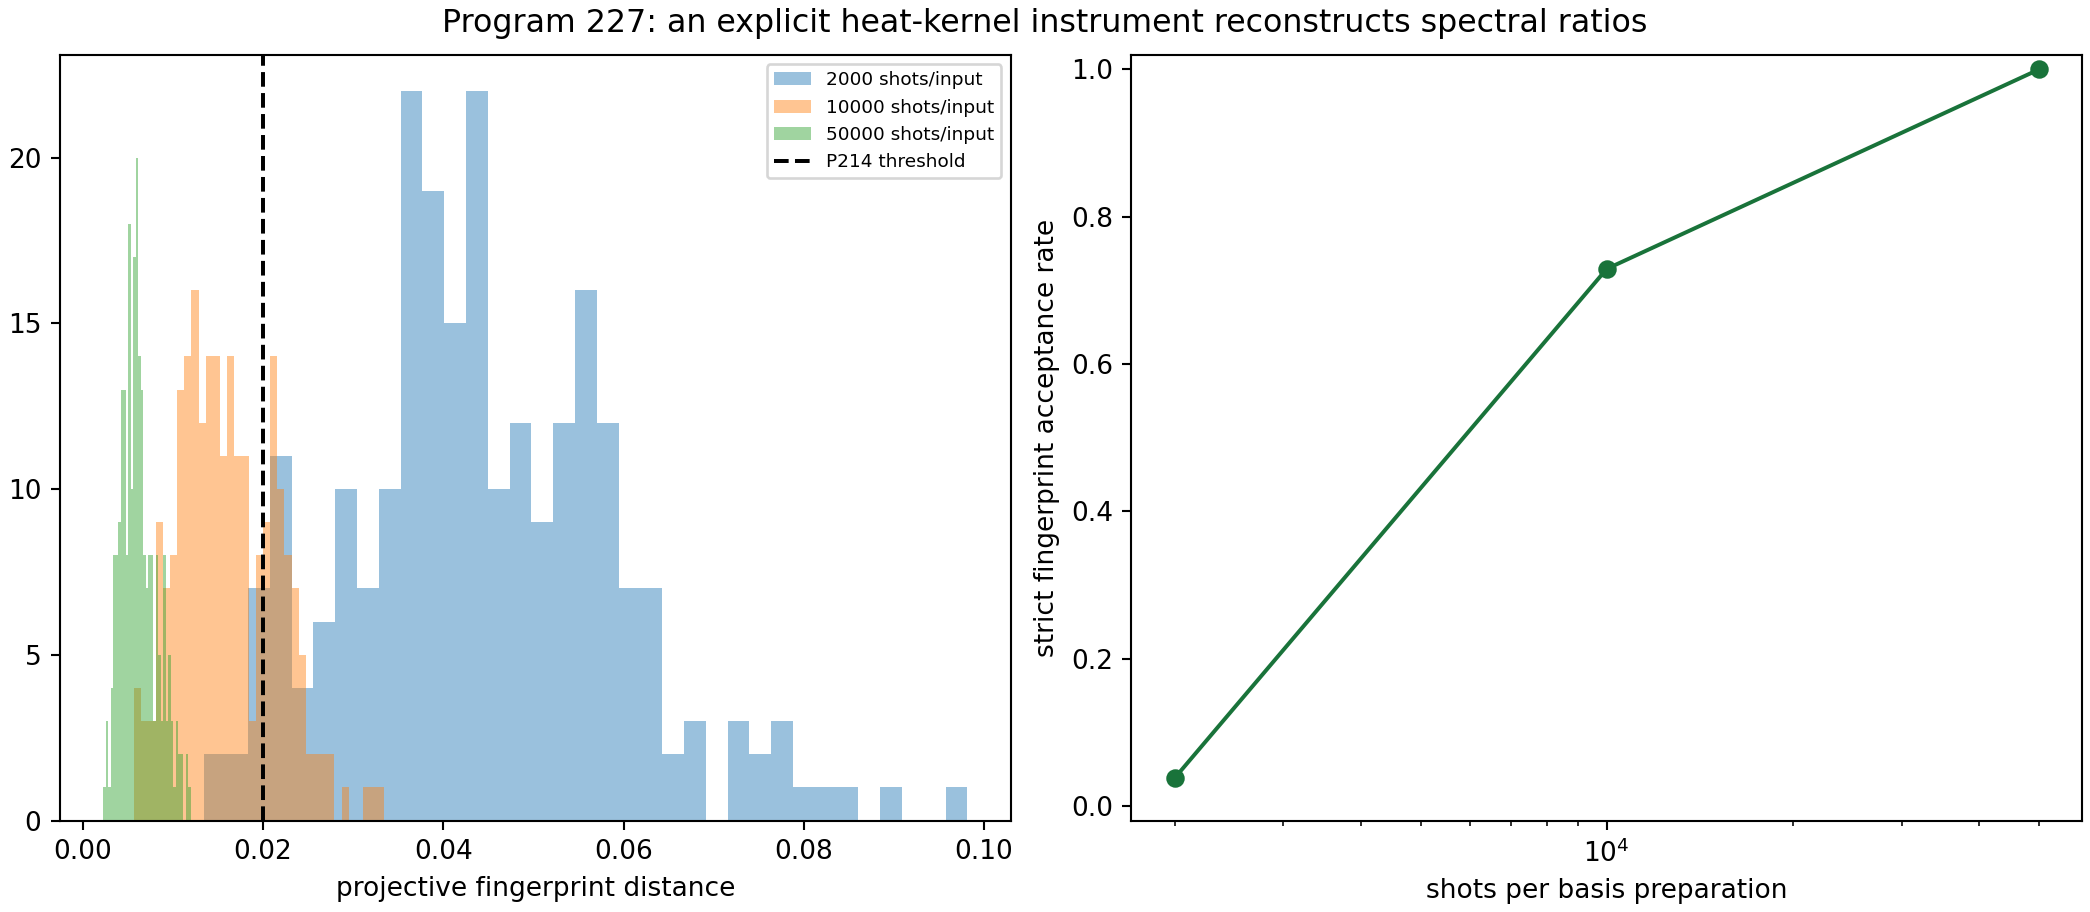
\includegraphics[width=0.94\textwidth]{FIN_Programs_217_229_Operational_Section_Spectral_Tomography_Figures/program227_spectral_tomography.png}
\caption{Finite heat-kernel transition counts reconstruct the projective strict spectral fingerprint with shot-dependent power.}
\end{figure}

\par\medskip\hrule\medskip

\chapter{Program 228 --- Independent custody and double-slit intake}

The revised eleven-field contract accepts either an ordered process record or an event-level double-slit record. It requires:

\begin{enumerate}
\item 
independent provider identity and license;

\item 
immutable raw-event hash;

\item 
ordered events or detection coordinates;

\item 
preparation or slit-configuration labels;

\item 
intervention or shutter-control labels;

\item 
clock and dimensional calibration;

\item 
detector geometry, efficiency, dark counts, and blur;

\item 
environment and background record;

\item 
negative controls;

\item 
a preregistered held-out target;

\item 
provider--registrar--analyst custody separation.

\end{enumerate}

A double-slit bundle must contain both-open, left-only, right-only, and both-closed runs with event coordinates, timestamps, configuration, and run identifier. A rendered image is not an event record.

The three local external-lineage candidates pass at most two fields. The synthetic method bundle passes ten but remains synthetic. No process or double-slit bundle is admitted. No web search or Firecrawl is used.

\textbf{Verdict --- Acquisition object constructed; empirical object absent.}

\begin{figure}[htbp]
\centering
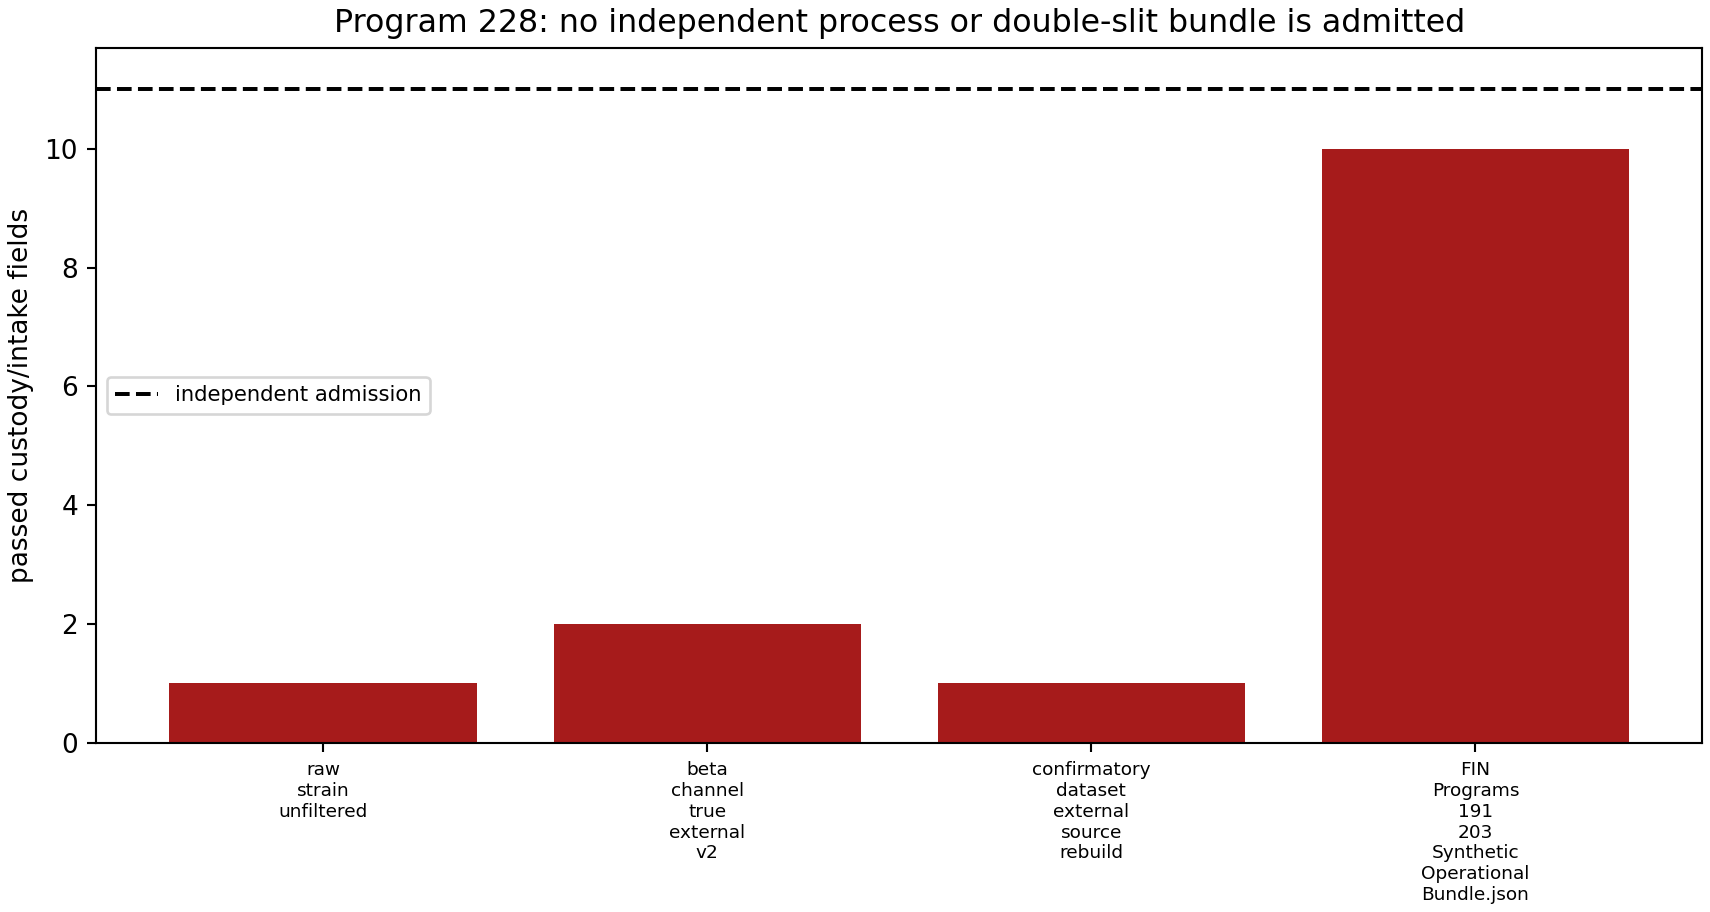
\includegraphics[width=0.94\textwidth]{FIN_Programs_217_229_Operational_Section_Spectral_Tomography_Figures/program228_external_custody.png}
\caption{No local process or event-level double-slit candidate passes the independent eleven-field custody gate.}
\end{figure}

\par\medskip\hrule\medskip

\chapter{Program 229 --- Registered semigroup holdout}

The frozen external test estimates \(P_\tau\) on a calibration subset and predicts

\[
P_{2\tau}^{\rm pred}=P_\tau^2.
\]

The primary statistic is the maximum column total-variation distance to the held-out \(P_{2\tau}\) record. The secondary statistic is the projective spectral fingerprint distance. Negative controls include time permutation, preparation-label permutation, the nearest-neighbour cycle, and the both-closed double-slit control when applicable.

The protocol may run once only after an immutable external bundle hash and custody-separated unblinding.

Program 228 fails, so Program 229 does not execute.

\textbf{Verdict --- Preregistered and locked.} The algebraic semigroup identity is not called an experimental success.

\begin{figure}[htbp]
\centering
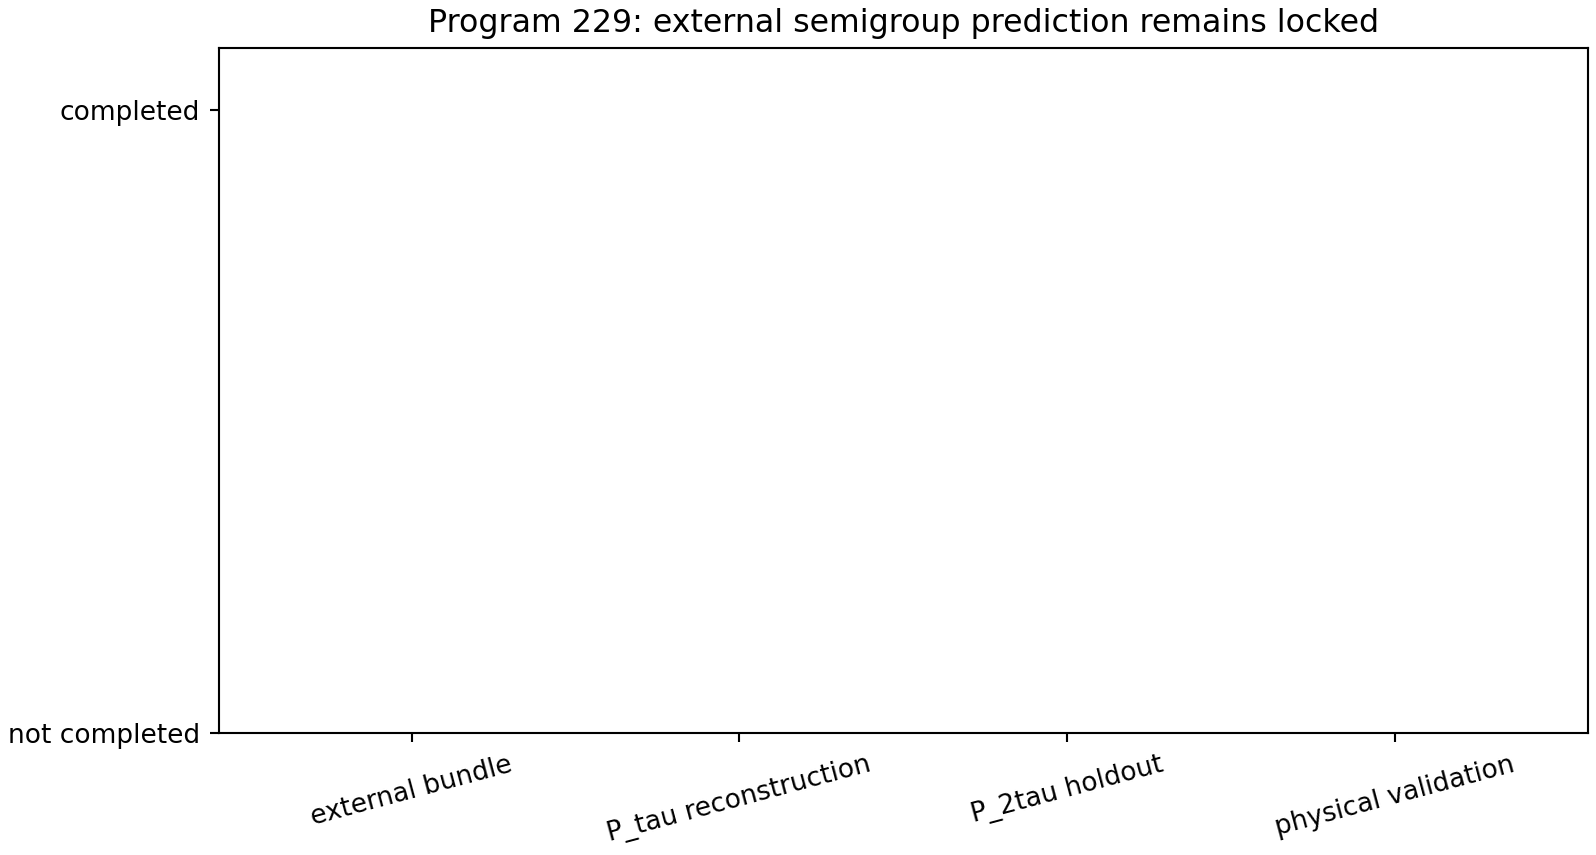
\includegraphics[width=0.94\textwidth]{FIN_Programs_217_229_Operational_Section_Spectral_Tomography_Figures/program229_prediction_lock.png}
\caption{The held-out semigroup prediction \(P_{2\tau}=P_\tau^2\) remains locked pending independent data.}
\end{figure}

\par\medskip\hrule\medskip

\chapter{Cross-program synthesis}

\section{The operational spectral section}

The round constructs the following conditional package:

\[
\mathfrak S_{\rm op}
=
(\rho,\mathcal P,\tau,\mathcal M,\mathcal R),
\]

where:

\begin{itemize}
\item 
\(\rho\) is a central state or preparation law;

\item 
\(\mathcal P\) is an informationally complete preparation family;

\item 
\(\tau\) is a clock reading;

\item 
\(\mathcal M\) is a measurement instrument;

\item 
\(\mathcal R\) is an ordered, independently sourced record.

\end{itemize}

Program 217 classifies \(\rho\) into invariant and preparation-selected cases. Program 227 supplies \(\mathcal P\), \(\tau\), and \(\mathcal M\) in a finite conditional model. Programs 228--229 specify the missing \(\mathcal R\) and held-out execution rule.

The operator \(A\) supplies none of these objects automatically. Once they are given, it makes sharp predictions.

\section{Selector as a finite reference resource}

Program 221 changes the selector discussion from a binary existence question to a resource theory:

\[
\text{asymmetry produced}
\quad\Longleftrightarrow\quad
\text{reference consumed, disturbed, correlated, or perfect}.
\]

The strict selector remains unsourced. Nevertheless, an operational theory can now record exactly which resource is used and where it goes. This is a constructive theoretical object, not merely a no-go statement.

\section{Information, diffusion, and observer records}

The heat semigroup contracts nonconstant modes, but an observer record is not the vector \(P_tf\) alone. It is a random record produced by preparation, environment, clock, and instrument. Programs 222--224 quantify how dependence, sequential stopping, finite shots, and misspecification change what may be inferred from that record.

The observer paradox is therefore resolved at the level of mathematical typing:

\[
\text{unitary and heat functions of }A
\ne
\text{a complete measurement theory}.
\]

There is no inconsistency between \(e^{-itA}\) and \(e^{-tA}\). There is an operational choice of experiment.

\section{Dimensional physics}

Program 227 recovers only

\[
\frac{\lambda_k}{\lambda_{\max}}.
\]

To recover dimensional eigenvalues, one must know a physical \(\tau\). To call \(\hbar A\) a Hamiltonian, one must additionally supply an action unit. To convert graph labels into length, one must supply a spatial calibration.

Thus the smallest current dimensional bridge remains a conversion package, not a number derivable from projective spectral geometry:

\[
{\rm CA}=(\tau_*,\ell_*,\hbar_*)
\]

or an equivalent independent basis of units. This package is selector-blind.

\section{Lagrangian status}

The quadratic action

\[
S[\phi]
=
\frac12\phi^\mathsf TA\phi-J^\mathsf T\phi
\]

still reconstructs the Green equation \(A\phi=J\). Program 227 now gives an operational route to estimate \(A\) conditionally. It does not derive the source \(J\), a physical action unit, tensor fields, or a full nonproxy Lagrangian. Existing reverse-closure obstructions therefore remain intact.

\section{Deepest surviving interpretation}

The strongest interpretation after Programs 217--229 is:

\begin{quote}\itshape
FIN is a dimensionless spectral-information theory whose internal operator admits a complete finite operational tomography theorem. The remaining transition to physics is a section problem: select a state, supply a finite symmetry reference or sector choice, calibrate a clock and units, realize preparations and measurements, and obtain an independent record. Exact mathematics now describes several of these obligations and proves that the others are not generated by affine, symmetric, or purely projective data.

\end{quote}

\par\medskip\hrule\medskip

\chapter{Falsification ledger}

\section{Results that survived}

\begin{itemize}
\item 
Uniform central weights are unique in the bistochastic/\allowbreak{}permutation category.

\item 
Preparation frequencies define a separate operational state.

\item 
Affine-natural exponent vector fields cannot select \(4/5\).

\item 
The finite C4 Lean certificate compiles.

\item 
Imperfect reference asymmetry cannot be broadcast with exact product return.

\item 
Correlated marginal return has a measurable information cost.

\item 
The robust mixing optimizer preserves its declared total failure budget.

\item 
Insertion ranks generate a rank-filtration e-process.

\item 
The third environmental moment interval is exact and sharp.

\item 
The finite torsion Lean certificate compiles.

\item 
Exact heat data uniquely determine the projective generator.

\item 
Finite shots show a real precision threshold for the spectral fingerprint.

\end{itemize}

\section{Results falsified or withheld}

\begin{itemize}
\item 
Bistochastic naturality is not a physical preparation theorem.

\item 
The strict exponent is not selected by natural autonomous flow.

\item 
The Arb certificate is not executed.

\item 
The general Mathlib theorem is not compiled.

\item 
The initial orientation sign is not sourced.

\item 
Naive fixed-calibration reuse lacks the required conditional e-value law.

\item 
The efficient tomography region is not exact finite-sample inference.

\item 
The finite phase core is not the full analytic formalization.

\item 
An intake contract is not a double-slit experiment.

\item 
The semigroup identity is not external validation.

\end{itemize}

\section{Robustness conditions}

Every result exposes its assumptions:

\begin{itemize}
\item 
change the morphism category and the invariant state may change;

\item 
add a non-affine scale-bearing datum and the exponent no-go may not apply;

\item 
consume another asymmetric source and the reference theorem requires a new resource balance;

\item 
violate the calibrated mixing envelope and the DKW design loses validity;

\item 
use score-dependent stopping and the rank-filtration proof no longer suffices;

\item 
leave the Gaussian visibility family and the likelihood region may be misspecified;

\item 
use a nonsymmetric or non-Markov transition matrix and the heat logarithm requires a different model;

\item 
omit custody separation and the record is not an independent replication.

\end{itemize}

\par\medskip\hrule\medskip

\chapter{Recommended Programs 230--242}

\section{Program 230 --- Experimental central-state preparation test}

Implement randomized sector permutations and a separately controlled nonuniform preparation law. Test whether observed frequencies follow the bistochastic invariant state or the apparatus preparation state.

\textbf{Primary object:} CentralStatePreparationExperiment.\\
\textbf{Success:} preregistered discrimination with calibrated confusion matrix.\\
\textbf{Probability of a useful operational result:} \(0.80\).

\section{Program 231 --- One-new-datum eta-flow classification}

Permit exactly one new strict-derived non-affine invariant \(q\) and classify all low-degree flows

\[
\dot x=F(x,q)
\]

that are equivariant, structurally stable, and do not contain \(4/5\) in their definition. If no repository-sourced \(q\) exists, issue a broader no-new-datum theorem rather than fitting the target.

\textbf{Probability of a strict source:} \(0.10\).\\
\textbf{Probability of a stronger no-go:} \(0.75\).

\section{Program 232 --- Authorized pinned Arb execution}

Obtain explicit authorization for one hashed Arb/\allowbreak{}FLINT environment, record the container digest and package versions, and execute all five frozen nodes. Do not change the \(0.03\) threshold.

\textbf{Probability after infrastructure access:} \(0.80\).

\section{Program 233 --- General Mathlib Dirichlet and heat library}

Pin Lean and Mathlib, repair the current general source, and formalize:

\begin{enumerate}
\item 
the Dirichlet identity;

\item 
positivity;

\item 
the constant kernel;

\item 
stochastic heat evolution;

\item 
finite-dimensional logarithmic reconstruction.

\end{enumerate}

\textbf{Probability of Dirichlet closure:} \(0.85\).\\
\textbf{Probability of all five in one round:} \(0.45\).

\section{Program 234 --- Multi-use finite-reference ledger}

Extend Program 221 to \(N\) sequential uses. Derive lower bounds on accumulated correlation, disturbance, recovery error, and reference distinguishability. Determine whether correlations can be recycled or must grow monotonically.

\textbf{Probability of a quantitative theorem:} \(0.75\).

\section{Program 235 --- Joint calibration/\allowbreak{}allocation optimum}

Given a fixed total experimental budget, optimize how many trials should calibrate \(p_0\) and how many should enter the target record. Include the one-sided calibration failure probability and thinning loss.

\textbf{Probability of a useful exact finite optimizer:} \(0.90\).

\section{Program 236 --- E-process under weak dependence}

Replace iid insertion-rank exchangeability by one explicit weak-dependence or covariate-shift class. Candidate routes are blockwise ranks, conditional randomization, or predictable betting with a certified density-ratio bound.

\textbf{Probability of a scoped theorem:} \(0.55\).

\section{Program 237 --- Exact finite-shot likelihood process}

Construct a likelihood-ratio e-process or exact inversion method for \((b,v,c)\) that retains finite-sample coverage while approaching the widths of Program 224. Include the fourth contrast as a simultaneous model test.

\textbf{Probability of meaningful width reduction:} \(0.65\).

\section{Program 238 --- Fourth and fifth moment hierarchy}

Given \((c_1,c_2,c_3)\) intervals, compute sharp semidefinite intervals for \(c_4\) and \(c_5\), identify sparse extremal measures, and quantify the number of operational contrasts needed to separate declared environment families.

\textbf{Probability of exact low-order results:} \(0.90\).

\section{Program 239 --- Full phase theorem in Lean/\allowbreak{}Mathlib}

Formalize continuous circle endomorphisms, the required automatic-continuity statement or an imported theorem with exact provenance, and the transcendence-based non-torsion result. Keep finite and analytic layers separate until all compile.

\textbf{Probability in one round:} \(0.35\).

\section{Program 240 --- Optimal spectral tomography design}

Optimize evolution times and preparation allocation for the projective fingerprint. Prove nonasymptotic matrix concentration bounds and compare one time with multiple-time designs.

\textbf{Probability of substantial shot reduction:} \(0.80\).

\section{Program 241 --- Blind-custody double-slit or process acquisition}

Obtain one event-level external bundle satisfying Program 228. Freeze the provider, registrar, and analyst roles before unblinding. A rendered interference image is insufficient.

\textbf{Probability:} determined by external coordination, not mathematics.

\section{Program 242 --- Single external semigroup execution}

If and only if Program 241 passes all fields, execute Program 229 once. Report the semigroup holdout, spectral fingerprint, all negative controls, and failure without post-hoc repair.

\textbf{Priority:} conditional but scientifically decisive.

\section{Ranked roadmap}

\begin{center}
\begingroup\small
\setlength{\tabcolsep}{3.5pt}
\renewcommand{\arraystretch}{1.16}
\begin{longtable}{@{}p{0.160\textwidth}p{0.280\textwidth}p{0.420\textwidth}@{}}
\toprule
\textbf{Rank} & \textbf{Program} & \textbf{Reason} \\
\midrule
\endhead
1 & 240 & directly improves the new instrument-to-spectrum bridge \\
2 & 241 & supplies the missing independent empirical object \\
3 & 234 & converts selector use into a quantitative multi-use law \\
4 & 238 & extends an exact environmental theorem \\
5 & 233 & closes the general formal operator library \\
6 & 237 & combines efficiency with rigorous finite-sample inference \\
7 & 235 & makes hidden-mixing acquisition economically meaningful \\
8 & 230 & tests categorical versus prepared central states \\
9 & 232 & closes long-standing numerical certification debt \\
10 & 236 & enlarges sequential validity beyond iid records \\
11 & 231 & high conceptual value but low strict-source probability \\
12 & 239 & valuable formal closure with substantial library cost \\
13 & 242 & decisive only after external admission \\
\bottomrule
\end{longtable}
\endgroup
\end{center}

\par\medskip\hrule\medskip

\chapter{Final conclusion}

Programs 217--229 construct several missing theoretical objects rather than renaming the remaining gaps.

The central state is now a precisely categorized section. The exponent obstruction is now an affine-natural no-go theorem. The selector is now a finite asymmetry resource with a no-broadcast law and a correlation ledger. The environment is now constrained by a second sharp moment interval. The operator is now connected to explicit preparations and measurements by a heat-kernel tomography theorem.

The smallest current operational bridge is

\[
(A;\rho,\mathcal P,\tau,\mathcal M,\mathcal R).
\]

The repository supplies \(A\). This round classifies or conditionally constructs \(\rho\), \(\mathcal P\), \(\tau\), and \(\mathcal M\). It does not supply the physical calibration of \(\tau\), a strict selector, or the independent record \(\mathcal R\).

Accordingly:

\begin{quote}\itshape
FIN has advanced from a dimensionless spectral generator with an informal measurement gap to a generator with a rigorous finite tomography theorem. It is still not a physical theory because the operational section has not been independently realized and dimensionally calibrated. The next scientifically decisive step is not another internal fit; it is optimal tomography followed by one blind-custody external execution.

\end{quote}

\par\medskip\hrule\medskip

\chapter{Reproducibility}

Run:

MPLCONFIGDIR=/\allowbreak{}tmp/\allowbreak{}matplotlib-fin217 \\
python3 fin\_programs\_217\_229\_operational\_section\_spectral\_tomography.py

MPLCONFIGDIR=/\allowbreak{}tmp/\allowbreak{}matplotlib-fin217 \\
python3 -m unittest -v \\
test\_fin\_programs\_217\_229\_operational\_section\_spectral\_tomography.py

The expected result is thirteen executed programs and 82 passing tests. The suite also directly invokes the local Lean compiler for two dependency-free sources and records the failed general Mathlib and Arb gates.

Suggested citation:

\.Zuchowski, K. (2026). \emph{FIN Programs 217--229: Operational Sections, Reference Costs, and Heat-Kernel Spectral Tomography} (FIN Research Monograph, Release 10.20; Version 1.0.0) [Preprint]. Zenodo.


\clearpage
\chapter*{Release reproducibility}
\addcontentsline{toc}{chapter}{Release reproducibility}
\begin{Verbatim}[fontsize=\small]
MPLCONFIGDIR=/tmp/matplotlib-fin217 \
python3 fin_programs_217_229_operational_section_spectral_tomography.py

MPLCONFIGDIR=/tmp/matplotlib-fin217 \
python3 -m unittest -v \
  test_fin_programs_217_229_operational_section_spectral_tomography.py
\end{Verbatim}

Machine-readable results are stored in
\path{FIN_Programs_217_229_Operational_Section_Spectral_Tomography_Results.json}.
The release contains five auxiliary contracts or formal records, two
machine-compiled Lean core sources, 82 tests, and thirteen figures.

\medskip
\noindent\textbf{Suggested citation:}

\.Zuchowski, K. (2026). \emph{FIN Programs 217--229: Operational Sections,
Reference Costs, and Heat-Kernel Spectral Tomography}
(FIN Research Monograph, Release 10.20; Version 1.0.0) [Preprint]. Zenodo.
\end{document}
